%
% exemplo genérico de uso da classe iiufrgs.cls
% $Id: iiufrgs.tex,v 1.1.1.1 2005/01/18 23:54:42 avila Exp $
%
% This is an example file and is hereby explicitly put in the
% public domain.
%
\documentclass[ppgc,mestrado,english]{inputs/iiufrgs}
% um tipo específico de monografia pode ser informado como parâmetro opcional:
%\documentclass[tese]{iiufrgs}
% monografias em inglês devem receber o parâmetro `english':
%\documentclass[diss,english]{iiufrgs}
% a opção `openright' pode ser usada para forçar inícios de capítulos
% em páginas ímpares
% \documentclass[openright]{iiufrgs}
% para gerar uma versão somente-frente, basta utilizar a opção `oneside':
% \documentclass[oneside]{iiufrgs}
\usepackage[T1]{fontenc}        % pacote para conj. de caracteres correto
\usepackage[utf8]{inputenc}   % pacote para acentuação
\usepackage{graphicx}           % pacote para importar figuras
\usepackage{times}              % pacote para usar fonte Adobe Times
\usepackage[version=3]{mhchem} 	% pacote para usar chemistry formulae
\usepackage{chemfig}
\usepackage{amsmath}
%\usepackage{biblatex}
\usepackage[alf,abnt-emphasize=bf,num]{abntex2cite}
\usepackage{amsthm}
\usepackage{amssymb}
\usepackage{mathtools}
\usepackage{multirow}
\usepackage{acronym}
\usepackage[acronym]{glossaries}
\usepackage{textcomp}
\usepackage{adjustbox}
\usepackage{array}
\usepackage{listings}
\usepackage{tablefootnote}
\usepackage{placeins}
\usepackage{booktabs}
\usepackage{pifont}



%\usepackage{mathptmx}          % p/ usar fonte Adobe Times nas fórmulas

%
% Informações gerais
%
\title{\emph{SHPECK} - A Geochemical Speciation Modelling Software}

\author{Damiani}{Leonardo Hax}
% alguns documentos podem ter varios autores:
%\author{Flaumann}{Frida Gutenberg}
%\author{Flaumann}{Klaus Gutenberg}

% orientador e co-orientador são opcionais (não diga isso pra eles :))
\advisor[Prof.~Dr.]{Dal Sasso Freitas}{Carla Maria}
\coadvisor[Prof.~Dr.]{Park}{Anthony J.}

% a data deve ser a da defesa; se nao especificada, são gerados
% mes e ano correntes
%\date{maio}{2001}

% o nome do curso pode ser redefinido (ex. para TCs)
%\course{Curso de Especialização em Cachaça}

% o local de realização do trabalho pode ser especificado (ex. para TCs)
% com o comando \location:
%\location{Itaquaquecetuba}{SP}

% itens individuais da nominata podem ser redefinidos com os comandos
% abaixo:
% \renewcommand{\nominataReit}{Prof\textsuperscript{a}.~Wrana Maria Panizzi}
% \renewcommand{\nominataReitname}{Reitora}
% \renewcommand{\nominataPRE}{Prof.~Jos{\'e} Carlos Ferraz Hennemann}
% \renewcommand{\nominataPREname}{Pr{\'o}-Reitor de Ensino}
% \renewcommand{\nominataPRAPG}{Prof\textsuperscript{a}.~Joc{\'e}lia Grazia}
% \renewcommand{\nominataPRAPGname}{Pr{\'o}-Reitora Adjunta de P{\'o}s-Gradua{\c{c}}{\~a}o}
% \renewcommand{\nominataDir}{Prof.~Philippe Olivier Alexandre Navaux}
% \renewcommand{\nominataDirname}{Diretor do Instituto de Inform{\'a}tica}
% \renewcommand{\nominataCoord}{Prof.~Carlos Alberto Heuser}
% \renewcommand{\nominataCoordname}{Coordenador do PPGC}
% \renewcommand{\nominataBibchefe}{Beatriz Regina Bastos Haro}
% \renewcommand{\nominataBibchefename}{Bibliotec{\'a}ria-chefe do Instituto de Inform{\'a}tica}
% \renewcommand{\nominataChefeINA}{Prof.~Jos{\'e} Valdeni de Lima}
% \renewcommand{\nominataChefeINAname}{Chefe do \deptINA}
% \renewcommand{\nominataChefeINT}{Prof.~Leila Ribeiro}
% \renewcommand{\nominataChefeINTname}{Chefe do \deptINT}

% A seguir são apresentados comandos específicos para alguns
% tipos de documentos.

% Relatório de Pesquisa [rp]:
% \rp{123}             % numero do rp
% \financ{CNPq, CAPES} % orgaos financiadores

% Trabalho Individual [ti]:
%\ti{123}     % numero do TI
% \ti[II]{456} % no caso de ser o segundo TI

% Trabalho de Conclusão [tc]:
% além de definir explicitamente o nome do curso (\course) e o local
% de realização (\location), é necessário redefinir a nominata,
% pois as informações necessárias dependem do curso. Ex.:
%\renewcommand{\nominata}{
%        UNIVERSIDADE FEDERAL DO RIO GRANDE DO SUL\\
%        Reitora: Prof\textsuperscript{a}.~Wrana Maria Panizzi\\
%        Pró-Reitor de Ensino: Prof.~José Carlos Ferraz Hennemann\\
%        Diretor do Instituto de Informática: Prof.~Philippe Olivier Alexandre Navaux\\
%        Coordenador do curso: Prof.~Seu Creysson\\
%        Bibliotecária-chefe do Instituto de Informática: Beatriz Regina Bastos Haro
%}

% Monografias de Especialização [espec]:
% \espec{Redes e Sistemas Distribuídos}      % nome do curso
% \coord[Profa.~Dra.]{Weber}{Taisy da Silva} % coordenador do curso
% \dept{INA}                                 % departamento relacionado

%
% palavras-chave
% iniciar todas com letras minúsculas, exceto no caso de abreviaturas
%
\keyword{Geochemical Modelling}
\keyword{Chemical Equilibrium}
\keyword{Geochemical Speciation}
\keyword{Water-Rock interactions}
\keyword{Multiphase System}
\keyword{Software Engineering}

\lstset{language=C++,
	basicstyle=\ttfamily\scriptsize,
	keywordstyle=\color{blue}\ttfamily,
	stringstyle=\color{red}\ttfamily,
	commentstyle=\color{green}\ttfamily,
	breaklines=true}
	
\renewcommand{\lstlistingname}{Code}

%
% inicio do documento
%

\newcolumntype{R}[2]{%
    >{\adjustbox{angle=#1,lap=\width-(#2)}\bgroup}%
    l%
    <{\egroup}%
}
\newcommand*\rot{\multicolumn{1}{R{50}{1em}}}% no optional argument here, please!
\newcommand*\OK{\ding{51}}


\begin{document}

% folha de rosto
% às vezes é necessário redefinir algum comando logo antes de produzir
% a folha de rosto:
%\renewcommand{\coordname}{Coordenadora do Curso}
\maketitle

% dedicatoria
\clearpage
\begin{flushright}
\mbox{}\vfill
{\sffamily\itshape
``To achieve great things, two things are needed:\\
 a plan and not quite enough time.''\\}
--- \textsc{Leonard Bernstein}
\end{flushright}

\renewcommand*\bibname{References}

% sumario
\renewcommand*\contentsname{Summary}
\tableofcontents

% lista de abreviaturas e siglas
% o parametro deve ser a abreviatura mais longa


\begin{listofabbrv}{SPMD}
\item[a] Activity
\item[ASCII] American Standard Code For Information Interchange
\item[CRUD] Create / Read / Update / Delete
\item[CPU] Central Processing Unit
\item[DBH] Debie-Hueckel 
\item[\ce{E_a}] Activation Energy
\item[Eh] Redox Potencial
\item[FLOPS] Floating-Point Operations per Second
\item[GUI] Graphical User Interface
\item[GWB] The Geochemist's Workbench
\item[HCI] Human-Computer Interaction        
\item[I] Ionic Strength
\item[IAP] Ion Activity Product 
\item[K] Equilibrium Constant        
\item[\ce{k_{diss}}] Dissolution rate constant
\item[\ce{k_0}] Pre-exponential (Arrhenius) factor
\item[LLNL] Lawrence Livermore National Laboratory
\item[m] Molality
\item[M] Molarity
\item[MVC] Model-View-Controller
\item[OS] Operating System
\item[pH] Power of Hydrogen
\item[R] Universal Gas Constant
\item[SI] Saturation Index 
\item[T] Temperature
\item[UI] User Interface
\item[USGS] U.S. Geological Survey
\item[$\gamma$] Activity coefficient
\item[$\beta_i$] Stability Constant         
\end{listofabbrv}


% idem para a lista de símbolos
%\begin{listofsymbols}{$\alpha\beta\pi\omega$}
%       \item[$\sum{\frac{a}{b}}$] Somatório do produtório
%       \item[$\alpha\beta\pi\omega$] Fator de inconstância do resultado
%\end{listofsymbols}

% lista de figuras
\listoffigures

% lista de tabelas
%\listoftables

% resumo na língua do documento


\renewcommand*\abstractname{Abstract}

\begin{abstract}    
%Chemical modelling is essential to comprehend many environmental problems.
%We present a flexible and general computer software, called \emph{SHPECK}, to calculate the geochemical speciation modelling dynamically and efficiently. 
%Geochemical modelling applications require an extremely high level of computations in a single simulation. 
%The method uses the stoichiometric approach (also known as law of mass-action approach) coupled with mass-action equations and a system of equilibrium constants solved using Newton's method. An adaptive control scheme of internal factors of the simulation is adopted to guarantee that chemical and physical processes are respected and follow the literature. 
%The software operates with customised options as capabilities to specify pH (activity of Hydrogen ions) of an aqueous solution, concentrations of the species, convergence criteria and maximal number of iterations. The proposed algorithm developed is described carefully from a software development point of view. 
%We present a comparison study about the existing geochemical modelling solvers. Finally, a study case using different solvers applied to the same system: evaporites (halite and sylvite) in an aqueous solution containing sodium (\ce{Na^+}), chlorine (\ce{Cl^-}) and potassium (\ce{K^+}). An application of this geological behaviour is the influence of the salt dome in turbidite reservoirs of oil and gas.
A geochemical speciation modelling software is responsible for calculating the distribution of dissolved species between solutes and aqueous complexes, and also computes saturation indexes for different minerals. In this work we introduce \emph{SHPECK}, a software developed to model geochemical equilibrium systems using the mass-balance conditions based on the phase rule concept \cite{Garrels:65}. 
\emph{SHPECK} composes a system of mass-action equations coupled with equilibrium constraints and solve using \emph{Newton-Raphson} method. Our software accepts any general combination of elements, species, and reactions, allowing the user to create different environments, simulations and, therefore, fully control any aspect and configuration of the model. It provides an interactive and intuitive user interface as well as the support of a built-from-the-ground database structure that handles the management of the whole thermodynamic data used for the geochemical modeling. 
Also, we present the basic concepts for geochemical modeling followed by a computer science based review about the available geochemical modeling software.
Finally, we validate \emph{SHPECK} by modeling the diagenetic reactions observed in a sandstones' reservoir and performing a comparative study with the previously discussed software. In addition to this, a database comparison was addressed and the results demonstrate a substantial improvement on the performance by the use of the \emph{SHPECK}'s relational database.
\end{abstract}




\newpage
% Introduction
\chapter{Introduction} 
\label{chapter:intro}

%PROBLEM

Geochemical modelling corresponds to the design of the reactions that occur in a geological structure through the usage of chemical properties (either thermodynamics and kinetics) to describe it. The need to understand the Earth's interior (both at high-temperature - magma - and low-temperature - aqueous solutions near the surface) motivates the effort in this area of study with the development of models and simulations. The applications of geochemical models are essential in several environmental problems, such as calculating the composition of natural waters, measuring flowing groundwater or surface water and the formation and dissolution of rocks and minerals in geologic formations. A geochemical speciation modelling software is responsible for calculating the distribution of dissolved species between free ions and aqueous complexes and also saturation indexes for different minerals. 

%DEFINITION OF MODELLING

A mathematical model, as described in \cite{Sarker:08}, requires three major components: decision variables (unknowns of the model); objective function (which needs to be optimized); and constraints (restrictions or limitation of the model). The decision variables depend on the type of the problem considered.  The objective function represents the goal of the problem in term of decision variables. The constraints are the restrictions or limitations of the problem.

As stated in \cite{Drever:05}, a chemical model is a theoretical construct that permits the calculation of chemical properties and processes, such as thermodynamics. Following this idea, a geochemical model is a chemical model developed for geologic systems. Geochemical models incorporate chemical models. A set of mathematical expressions represents these natural processes and handle modelling the system. The thermodynamics and kinetics data used to establish the reactions and mimic nature are directly responsible for the accuracy and precision of the geochemical model.


%THIS WORK - MOTIVATION/CONTRIBUTION

In this work, we develop a software that through the stoichiometry formulation calculates the chemical equilibrium of a geochemical system using the approach of imposing mass-balance conditions according to the species of the system. This process is known as chemical speciation, and the software was named as \emph{SHPECK}. It accepts any general combination of elements, species and reactions, allowing the user to create different environments, simulations and, therefore, fully control any aspect and configuration of the model. Also in this work, we show a thorough analysis of the available existing solutions, and we made clear the uniqueness of our computational approach to the geochemical modelling problem. 

Using a high-level and object-oriented programming language, we could implement an efficient solution that models geochemical speciation. \emph{SHPECK} provides an interactive and intuitive user interface - unique among geochemical speciation software - as well as the support of a built-from-the-ground database structure that handles the management of the whole information used by \emph{SHPECK}. These two contributions are presented as the result of an extensive study about the available software normally in use to perform geochemical speciation simulations.Their flow of information (input and output) are old, complexes and prone to error. It is also important to mention that these software fetch the information from flat file databases. Both of these characteristics are responsible for frequent errors, problems and wrong interpretations.

%BASIC CONCEPTS USED

The principles of chemical equilibrium calculation rely on the law of conservation of mass (also known as the principle of mass conservation), stated by Antoine Lavoisier, and chemical speciation, which was presented by Garrels and Christ  \cite{Garrels:65}. 
The law of conservation of mass establishes that the total mass of an isolated system will remain constant and is independent of any chemical and physical changes taking place within the system. Therefore, the challenge of chemical equilibrium calculations is finding the number of moles that satisfies a system of equilibrium constraints at the moment where forward and reverse reactions rates are the same. 
These constraints are organized in a form of linear conservation equations, which may be expressed in the form of either linear algebraic atom and charge balance equations or chemical equations \cite{SmithMissen83}. For the sake of simplicity, in this work we will only deal with chemical equilibrium and not with chemical kinetics calculations since the first one requires only the solution of algebraic equation. It is planned to integrate kinetics reactions in the future.

%APPLICATION

The system of equations will drive and represent all the interactions between the components of the simulation. Newton-Raphson's method uses the previous guess for the equilibrium calculation in a subsequent step, recursively, until finding a suitable solution that satisfies the system and the convergence criteria. 
One must note that the initial guess is generated automatically and used as a seed for the iterations. This method requires the usage of a Jacobian matrix and a residual vector during the algebraic calculations. Geochemical modelling speciation has an important application in processes that occur in turbidite reservoirs. 
The process of the water coming from a salt dome contains a high concentration of salts as sodium (\ce{Na^+}), chlorine (\ce{Cl^-}) and potassium (\ce{K^+}). Compactation, cementation, dissolution or recrystalization can be observed inside turbidites when this process happens. These processes might change drastically, for example, the porosity of the rock and, therefore, the storage capacity of oil and gas.

%OBJECTIVES OF THIS WORK
\section{Objectives of this work}
%This work has as purpose two main objetives:
%\begin{enumerate}
%\item Emphasize the importance of geochemical speciation modelling and make %explicit the need and uniqueness of the new software developed - \emph{SHPECK}. It %is a contribution to the geochemical modelling community by the adoption of a %structured Computer Science approach.
%\item Analysis, comparison, evaluation of the accuracy of the implemented software %with the available commercial options as well as demonstrate the advantages of %\emph{SHPECK} towards these options.
%\end{enumerate}
%\subsection{Emphasize the importance of geochemical speciation modelling}
Soils and aquifers are heterogeneous, subsurface systems composed of a large number of components - dissolved salts, minerals, metals, gases, natural organics, microorganisms, animals and plants. The subsurface is one of the most complex systems studied by scientists and engineers today. Because of this, geochemical modelling has gained importance and is being accepted as a useful tool to interpret subsurface geochemical processes. Geochemical speciation is based on thermodynamics concepts and the assumption of chemical equilibrium in geochemical reactions.
%\subsection{Implementation and validation of \emph{SHPECK}}
The idea of our own geochemical speciation software has emerged as an application where it would be possible to apply all the physical, chemical aqueous, geochemistry and linear algebra concepts, and develop a useful tool with an intuitive and interactive user interface. 
The most usual approach found in the area of geochemical modelling is a geochemical expert that develops a solution to solve his/her particular problem and generates a specific code/algorithm - a solution that most of the times is not very reliable and has no scalability. 
In this work, the approach was for the computer science expert to made the necessary efforts to understand and learn all the complex aspects of a geochemical speciation model and develop a software based on a solid knowledge in computer architecture, algorithms and software engineering. 

The main purpose of this work is to develop a geochemical speciation modelling software following a structured computational approach. 


%STRUCTURE OF THIS WORK - TO BE VERIFIED AT THE END OF THE WORK
The rest of this work is structured as follow. In chapter 2, we present an overview of the basic concepts needed and technical concepts involved in this work. Chapter 3 shows a thoroughly analysis and review of the commercial software available. Chapter 4 presents the \emph{SHPECK} implementation with a detailed description of the whole system: design options; mathematical treatment and details; implementation and user interface (UI) details; algorithm validation and complexity; architecture and organization of the software as well as the database; data-flow; and iteration control. In Chapter 5, it is presented a study case with an interesting and relevant scenario; the results that validate \emph{SHPECK} and a broad comparison between solutions previously addressed in this work. Chapter 6 brings the conclusion of this work. Finally, this work contains an Appendix A, which is a presentation and an analysis of a linear algebra library used for the development of \emph{SHPECK} called \emph{Armadillo C++}. -- THIS NEEDS TO BE VERIFIED LATER
\newpage
%%%%%%%%%%%%%%%%%%%%%%
%                                                                %
% BASIC CONCEPTS INTRODUCTION   %
%                                                                %
%%%%%%%%%%%%%%%%%%%%%%
\chapter{Basic Concepts for Geochemical Modelling}
\label{chapter:basic}

Applying Computer Science to solve problems and create solutions in different areas requires redefining obstacles outside normal boundaries and generating a new understanding of complex situations by thinking across two or more academic disciplines. 

To develop this work, we had to delineate common goals for the different profiles that would take part on it, all of them with a clear view of their roles and with a noiseless communication in any direction. Although for the completeness of the text we should have included an introduction to the computer science aspects involved in building the geochemical modeller, we restrain ourselves to introduce the basic concepts of the application domain, i.e., geochemistry. The computational concepts and tools used in the development are addressed in Chapter~\ref{chapter:SHPECK}

In the next section, we explain the essential hydrogeochemistry principles: an introduction to thermodynamics; and hydrochemical processes; And to finish, we focus on the geochemical modelling with a special section for it. If the reader feels comfortable with these topics, we recommend that you proceed to Chapter ~\ref{chapter:review}.


% BASIC CONCEPTS COMPUTER SCIENCE 
%\section{Computer Science Principles}
%\subsection{Computer Processing and Modelling}
%A processor is a small chip that resides in computers and electronic devices. Its job is to receive input, do something with it and provide the appropriate output. Modern processors, whose location is inside the \emph{central processing unit} or \emph{CPU}, can handle trillions of calculations per second and even work together to solve complex instructions. Within that \emph{CPU} is an electronic clock responsible for creating series of synchronized electrical pulses. These pulses are the key to integrating all the computer's components and perform calculations with the data pulled from the memory. In 2013 the supercomputer \emph{NUDT Tianhe-2} performed $33.86 Pflops$. $Pflops$ stands for Peta Floating-Point Operations Per Second and is the regular unit to measure computer performance.
%Nowadays, human's power of abstraction and modelling is what set the boundaries of the application and systems that we build. Countless factors influencing and driving the process are not a problem anymore for the computing power of the machines that are available. Not many years ago the bottleneck was on the computing power.

%The advances in computer processing made possible scientific modelling, which generates part or feature of the real world to understand, define, quantify, visualize or simulate \cite{Humphreys:04}. Modelling such systems require a previous knowledge of all the characteristics, the behavior of this domain and what is the goal of this modelling allied with a big \emph{"piece"} of abstraction. Popular models are, for example, conceptual models, operational models, mathematical models, graphical models. The advantages of a model are: help us to communicate; allow us to clarify and test understanding; create credibility and accountability; organize the thoughts; simplify and solve problems;

%The series of "orders" clearly expressed by the modeller is what defines the model. These stack of "orders" are known as algorithms - a series of instructions for how to do something. Instructions that tell the computer how to make decisions and when to do calculations - which are different according to the type of model.

%Among the many computer science areas, there is one that studies the complexity of algorithms. As algorithms are programs that perform a series of instructions, complexity analysis allows us to measure how fast a program is when it performs computations. The analysis enables us to explain how an algorithm behaves in the worst case scenario, for instance.
%This information will come in hand when we analyze the complexity of \emph{SHPECK}'s algorithm on chapter ~\ref{chapter:SHPECK}.

%SOFTWARE ARCHITECTURE AND DESIGN
%\subsection{Software Architecture and Design}
%WHAT IS SOFTWARE ARCHITECTURE
%Software Architecture is the process of finding a structured solution that achieves all of the technical and operational requirements also addressing attributes as performance, security, value for the user and management. The architecture and design of software are the \emph{art} of considering all of the several factors and tracing the best path available. Without compromising the impact on quality, interface, database structure, performance, maintainability and success of the software.

%The software architecture is responsible not only for the algorithms and the data structure but also by the organization, communication, synchronization, functionality and design of the desired elements, scaling and performance. There is no well-defined recipe for a good software architecture - it takes time, practice and efforts to start taking the right paths and weighing the options according to the needs. Recognizing paradigms and building relationships among systems can be a handful tool to perform successfully as a software architect.
%The software architect is responsible for structuring the software with a consolidated and dense foundation - anything other than this implies a risk for the application. Studying the scenarios and requirements before designing the application is a must. Poor architecture results in deployment problems, instability, lack of support and the complete failure of the software (sometimes even the entire business).
%GOALS OF SOFTWARE ARCHITECTURE
%A software architect aims to: 
%\begin{itemize}
%\item Catalog all the requirements of the application, as well as the use cases and scenarios;
%\item Analyze and reduce the risk either for the application and for the business (if there is one involved);
%\item Be able to adapt the design decisions around the reality - that will most likely change over time;
%\item Develop a structure where the tradeoffs of all attributes are clear and the impact of any change will be controlled;
%\end{itemize}

%During the development of \emph{SHPECK}, we adopt the Object-Oriented, also know by its abbreviation \emph{OO} or \emph{OOP}, architectural style. \emph{OO} is a paradigm based on the division of responsibilities into reusable and self-sufficient objects, each one of them containing the data and the behavior desired to its functionalities and responsibilities.
%For the purpose of illustration we listed a few other important architectural styles: client/server; domain driven design; service-oriented architecture (SOA);

%Before defining the architecture of \emph{SHPECK}, we have analyzed points as attributes, application type, technologies and deployment options. Only after this section was possible to identify which of the design architectures would fit best to our needs - small refinements were done along the way (which is normal).

%PRINCIPLES OF SOFTWARE ARCHITECTURE
%\subsubsection{Software Architecture Principles}
%The origin of software architecture principples is the need to minimize costs, address properly maintenance requirements and promote the \emph{Seven Basic Principles of Software Engineering} as in \cite{Boehm:83}, which are:
%\begin{enumerate}
%\item Manage using a phased life-cycle plan;
%\item Perform continuous validation;
%\item Maintain disciplined product control;
%\item Use modern programming practices;
%\item Maintain clear accountability for results;
%\item Use better and fewer people;
%\item Maintain a commitment to improve the process;
%\end{enumerate}
%Along these principles, it is mandatory that the software architect or designer to see the large picture of the software that is under his management. The large picture is responsible to make sure that no feature is overlaping (nor duplicating) with another - this will lead to a low coupling and highly cohesive software. 

%\subsubsection{Design Principles}
%Designing software is composing a structure with different layers responsible for various tasks or properties. This layering must be consistent with any operation and must respect the hierarchy as well as the orientation of this structure.
%These layers must be connected but never overlapping themselves: duplicating properties/functionalities/responsibilities is a mistake and prone to error. Overlapping layers is the signal of potential inconsistencies and elevated software maintenance costs. Design patterns are also one important term to keep in mind. Establishing a coding style, naming standards and conventions provide a consistent model that will make the software's life longer and more adaptable.

%SOFTWARE DEVELOPMENT 
%\subsection{Software Development}
%Software development is a process that requires extremely careful planning and execution to meet the proposed goals. The proposed goal is software, but sometimes people forget that to achieve this goal is necessary many hours of computer programming, documenting, testing, bug fixing and decisions making. Software development may also include research, new development, prototyping, modification, reuse, re-engineering and maintenance. The following sections discuss the most interesting and relevant points.
%LIFE CYCLE
%\subsubsection{Life Cycle of a Software Development Projet}
%This topic is relevant to clarify that lots of work are done before writing any line of code. We can mention tasks as requirements definition; functional specification; architecture and design decisions; implementing and testing; software deploy; documentation; and maintenance;
%There may be additional functions according to the reality of each software development, but the idea of life cycle must be a clear notion in the reader's mind.

%SOFTWARE ENGINEERING
%\subsubsection{Software Engineering}
%The contrast in time doesn't destroy the importance of software engineering among different periods as can be verified in the following quotes:
%\begin{itemize}
%\item \emph{``The establishment and use of sound engineering principles in order to obtain economically software that is reliable and works efficiently on real machines.''}, from \cite{Bauer:68}. 

%\item \emph{``Software engineering is the application of a systematic, disciplined, quantifiable approach to the development, operation, and maintenance of software, and the study of these approaches; that is, the application of engineering to software.''} by the \emph{IEEE Computer Society's Software Engineering Body of Knowledge} from 2004.
%\end{itemize}
%The understanding that overlaps in both quotes is that to achieve a proper \emph{software}, engineering principles (for example management issues, documentation, infrastructure, directing teams, scheduling and budgeting) are necessary and will be fundamental to reach that goal.

%DATABASE
%\subsubsection{Database}
%The database is responsible for organizing, storing and retrieve the data so it can be used efficiently and smoothly. A collection of schemes composes it in a way that it supports processes requiring information that are utilized by the application's internal operations. They are organized according to their approach: relational database; tabular database; distributed database; OO database; and flat file database;

%Among several types of database, the software engineering previously done should identify which of them suits better the needs of the software. Details of \emph{SHPECK}'s database are presented in chapter ~\ref{chapter:SHPECK}.

%USER INTERFACE
%\subsubsection{User Interface (\emph{UI}) and Human-Computer Interaction (\emph{HCI})}
%Psychology, ergonomics, engineering, graphic design and others fields of study influence the \emph{UI} and \emph{HCI} areas from computer science. Both areas take into account and are products of how humans interact with computers.

%Good \emph{UI} are not user-expensive nor task-expensive, they behave naturally as the extension of the user's needs and desires. The software will easily bring more value to its users if the \emph{HCI} happens in a mutually beneficial way - by reaching the software's goal and not being an embarrassment or annoyance for the user. Losses of productivity, efficiency, money and usability are expected consequences from a software that has skipped the preparation parts to the development of \emph{UI} and \emph{HCI}.

%\emph{UI} and \emph{HCI} were extensively studied and analysed along the development of \emph{SHPECK}.

% BASIC CONCEPTS HYDROGEOCHEMISTRY PRINCIPLES
\section{Hydrogeochemistry Principles}
% INTRODUCTION TO THERMODYNAMICS
\subsection{Introduction to Thermodynamics}
In thermodynamics, equilibrium is a state of dynamic balance where the ratio of the product and the reactant concentration is constant. There are three general approaches to calculating the composition of a solution at equilibrium \cite{Petrucci}.
\begin{enumerate}
    \item Manipulation of equilibrium constants (\emph{K}): The final concentrations are achieved by mathematical handling of the equilibrium constants; the idea is to express all the parts in terms of the measured equilibrium constant and initial conditions. Thermodynamics databases contain the values for the equilibrium constants obtained through experiments. Demonstration of this can be found in \cite{Kehew:00}. The disadvantage of this method is that it may never converge when using this method for a huge number of reactions.
    \item Gibbs Energy of the system: At equilibrium, the Gibbs Energy (G) is at a minimum. When the object of the study is a close system - no particles neither entering nor leaving - the total number of atoms of each element will remain constant, therefore, achieving the minimum free energy. Due to the complexity in demonstrating how this method works, it will be suppressed here. An interesting algorithm for equilibrium calculation that uses Gibbs energy is described in \cite{Allan:15}. One of the disadvantages of this method lies in the effect of species that appear only in tiny quantities at equilibrium.
    \item Manipulation of mass-balance: The total concentration of species that compose the system is the basis for this method. Smith \cite{Smith:80} explains this stoichiometric formulation approach. This method takes into account the stoichiometric approach among the species, which generates a system of non-linear mass-action equations. Mass-balance manipulation is the method chosen for this work, and the details are explained further in this text.
\end{enumerate}

Stoichiometric approaches have two general advantages over non-stoichiometric: in the case of real systems and for multiphase problems - in which singularities can occur in the linear equations \cite{Smith:80}. It is important to remind that all the methods described above are equivalent, and can be verified in \cite{Zeggeren:70}.

It is also important to mention that any analysis resulting from a water sample must be carefully taken. Any geochemical investigation is useless if the integrity of the water or the solid phase is compromised. Results of interpretation and modelling might be incorrect if the sampling was not done properly. A main objective is to obtain a water sample with the same chemical composition as that of the water in its original environment, for example, an aquifer or a surface water \cite{Deutsch:97}.

% THERMODYNAMIC EQUILIBRIUM
\subsubsection{Thermodynamic Equilibrium Reactions}
There are mainly two ways to describe thermodynamic equilibrium reactions: Equilibrium and Kinetic. Both of them formulate a closed system and describe the position of the maximum thermodynamic equilibrium. Equilibrium is the moment where there is no more chemical energy to alter the distribution of mass between reactants and products in the system. The way to model a reaction depends on its rate: an equilibrium reaction is relatively fast on the mass transport process, while the kinetic reaction is slow. Therefore, when applying an equilibrium model to a reaction, it is assumed that the whole mass transfer happens at the same time when the reactant and product are put together, and this will configure an equilibrium situation. If the reaction rate is slow, it requires a kinetic description of the reaction. In this work, we will address equilibrium reactions \cite{Nordstrom:86}. 

Assuming the independent equilibrium reactions:
\begin{equation}\label{reaction}
0 \ce{<=>} \sum\limits_{i=1}^N  v_{ji} \alpha_i \hspace{35pt}    (j = 1, ... , M)
\end{equation}
where $v_{ji}$ is the stoichiometric coefficient of the \emph{i-th} species in the \emph{j-th} reaction; and $M$ represents the number of reactions and $N$ the number of species, with $M < N$. The sign convention is to assign the stoichiometric coefficient negative for reactants and positive for products. Assuming that all the reactions in the system are in equilibrium, the chemical system must also satisfy the mass-action equations:
\begin{equation}\label{eq:massaction}
K_j =  \prod\limits_{i=1}^N  a_i^{v_{ij}} \hspace{35pt}    (j = 1, ... , M)
\end{equation}
where $K_j$ denotes the equilibrium constant of the \emph{j-th} reaction; $a$ denotes the activity of the \emph{i-th} chemical species. The equilibrium constant depends on the temperature of the system; therefore, the equilibrium constant needs to be calculated according to the temperature of the system. 

It has been known that the driving force of a chemical reaction is related to the concentration of the constituents that are reacting and the concentrations of the products of the reaction. The law of mass-action states that any reaction will proceed to the right (dissolution) or to the right (precipitation) until the mass-action equilibrium is achieved, being important to keep in mind that it may take years or even thousands of years for that equilibrium to be achieved and after a disturbance in the system, such as an addition of reactants, removal of products, changes in the temperature or pressure, the system will continue to proceed towards this new equilibrium (if the disturbances are frequent compared to the reaction rate, equilibrium will never be achieved) \cite{Freeze:79}. Each of the dissolved species will have one representation of the nonideal behavior of components in the solution, which is called \emph{activity} and is presented in details later on in this chapter.

Kinetic descriptions are applicable to any reaction but it is necessary to describe  reactions that are slow in relation to mass transport.  The following reaction has a $k_1$ and $k_2$ rates for the forward and reverse reactions, respectively 
\begin{eqnarray}
aA + bB \underset{k_1}{\overset{k_2}{=}} dD + eE 
\end{eqnarray}
Each ion has a reaction rate related to the stoichiometry, and is expressed as
\begin{eqnarray}
-\frac{r_A}{a} &=& -\frac{r_B}{b} = \frac{r_D}{d} = \frac{r_E}{e}
\end{eqnarray}
where $a, b, d$ and $e$ are stoichiometric coefficients of each one of the ions in the reaction. $r_A, r_B, r_D$ and $r_E$ are reaction rates, and they describe the time rate of change of concentration as function of rate constants and concentration. Each one of them express the rate of change at the chosen ion as the difference between the rate at which the component is being used in the forward reaction and generated in the reverse reaction and is described as follow
\begin{eqnarray}
r_A &=& - k_1 (A)^{n1}(B)^{n2} + k_2 (D)^{m1}(E)^{m2}
\end{eqnarray}
where $n1, n2, m1$ and $m2$ are empirical stoichiometric coefficients. When there are reactions in parallel or series the rate laws are even more complex.
The dissolution rate constant (\ce{k_diss}) of a chemical reaction depends on temperatue. The relation between constant and temperature is given by the \emph{Arrhenius equation}, described as
\begin{eqnarray}
k_diss = A * exp(\frac{-E_a}{R*T})
\end{eqnarray}
where \ce{k_0} is the pre-exponential (Arrhenius) factor, $E_a$ is the activation energy, R is the universal gas constant, and T is the temperature in Kelvin.
During the development of \emph{SHPECK}, we will not deal with kinetic reactions.

%EQUILIBRIUM CONSTANT
\subsubsection{Thermodynamic Equilibrium Constant}
The \emph{equilibrium constant} (\emph{K}), also known as \emph{stability constant}, is the value of the reaction quotient when the reaction has reached equilibrium, as stated in equation ~\ref{equilibrium_reaction}. \emph{K} depends only on the temperature and on the ionic strength of the solution. According to known reactions' equilibrium constant value, it is possible to determine the value for at any temperature by a polynomial fitting technique or polynomial regression.

Equilibrium constants are determined by measurements of the relevant concentrations of the species under differing experimental conditions. Concentrations of species can be measured in multiple ways, and the use of these values in modelling requires adjustment to the conditions in the system being modelled. These adjustments, as well as the differences in conditions and different methods for determination, can lead to uncertainty in chemical speciation constants.

Several thermodynamics database are available nowadays. They include reaction constants, reaction descriptions, solutes, species, enthalpy values, activity coefficient parameters, etc. During the development of \emph{SHPECK} we selected the \emph{Geochemist's Work Bench's} (\emph{GWB}) database - it contains also the values of a $8^{th}$ degree polynomial, which allows the user to calculate the equilibrium constant to any temperature. Also another source of data used along this work is \cite{Palandri:04}.

In geochemical modelling, polynomial regression is specifically used to calculate the equilibrium constant of the compound at the desired temperature. 
Polynomial regression is one of several methods of curve fitting, which is a process of constructing a curve that has the best fit to a series of data points. Polynomial regression is a statistic method that is a form of linear regression in which the relationship between the independent variable \emph{x} and the dependent variable \emph{y} is modelled as an \emph{nth} degree polynomial. In our case, the polynomial regression is necessary in order to obtain the equilibrium constant for compounds found in the solution system.

%Polynomial regression is considered to be a special case of multiple linear regression. A polynomial is a function that takes the form 

%\begin{equation} \label{eq:polynomialForm}
%f(x) = c_0 + c_1 * x + c_2 * x^2 + ... + c_n * x^n
%\end{equation}

%where \emph{n} is the degree of the polynomial and \emph{c} is a set of coefficients. Polynomial regression models are usually solved using the method of least squares. Likewise performing polynomial regression with a degree 0 on a set of data returns a single constant value. It is the same as the mean average of that data. This makes sense because the average is an approximation of all the data points, as shown in figure \ref{fig:degree0}. The average line mostly follows the path of the data points. Thus the mean average is a form of curve fitting and likely the most basic.

%\begin{figure}[ht!]
%\centering
%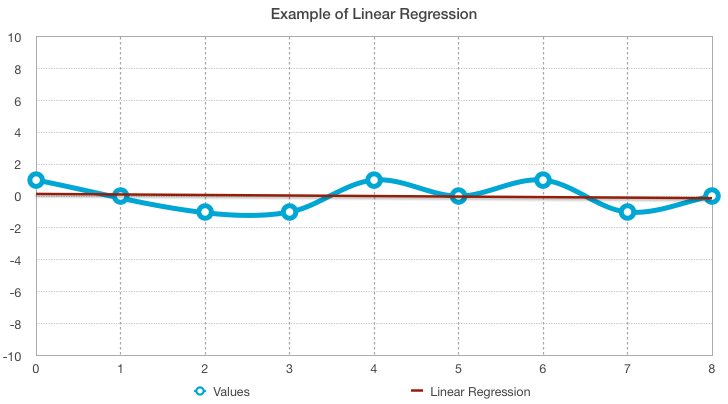
\includegraphics[width=100mm]{images/degree0.png}
%\caption{Example of Linear regression}
%\label{fig:degree0}
%\end{figure}

%Linear regression is polynomial regression of degree 1, and generally takes the form

%\begin{equation} \label{eq:polynomialFormSmall}
%f(x) = c_0 + c_1 * x
%\end{equation}

%where \emph{$c_0$} is the y-intercept and \emph{$c_1$} being the slope. Figure \ref{fig:degree1} shows clearly that the linear regression line running along the data points approximate the data. Mean average and linear regression are the most commom forms of polynomial regression, but not the only.

%\begin{figure}[ht!]
%\centering
%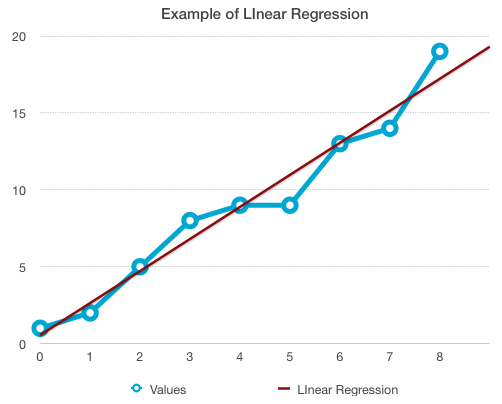
\includegraphics[width=100mm]{images/degree1.png}
%\caption{Example of Linear regression}
%\label{fig:degree1}
%\end{figure}

%The next step of polynomial would be the quadratic regression, now the regression becomes non-linear and the data is not restricted to straight lines. With figure \ref{fig:degree2} is possible to visualize a data with a quadratic regression trend line. Basically, the idea is simple: find a line that best fits the data which is find the coefficients to a polynomial that best fits the data.

%\begin{figure}[ht!]
%\centering
%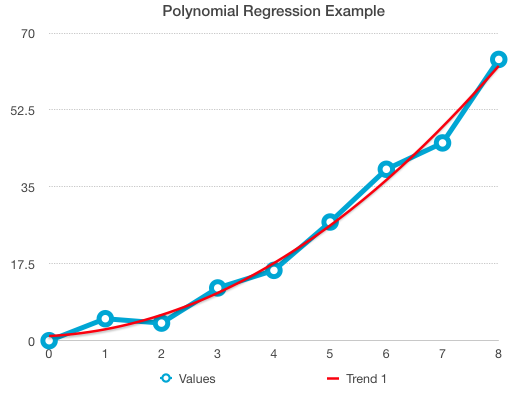
\includegraphics[width=100mm]{images/degree2.png}
%\caption{Example of Polynomial Regression}
%\label{fig:degree2}
%\end{figure}

%Polynomial regression is an overdetermined system of equations that uses least squares as a method of approximating an answer. To understand this, some linear algebra is required. 


%ACTIVITY OF A SOLUTE
\subsubsection{Activity of a solute}
Activity (\ce{a_i}) is \emph{"thermodynamic concentration"} (or informally known as \emph{"effective concentration"}). It is calculated as a product of activity coefficient and concentration (where \emph{i} means the solute involved):
\begin{equation}\label{activityEq}
a_i = \gamma_i * m_i
\end{equation}
Activity coefficient ($\gamma_i$) is a function of ionic strenght (I), which is a measure of the concentration of ions in the solution.  

%IONIC STRENGTH
\subsubsection{Ionic strength}
Mathematically the ionic strength of the solution is calculated according to
\begin{equation} \label{eq:ionicStrength}
I = 0.5 \sum{M_i z_i^2}
\end{equation}
where \emph{M} is the molar concentration of the specie \emph{i} having a charge \emph{z}.When \emph{I} increases, activity coefficients decrease. In very diluted solutions, activity coefficient is equals to \emph{1.0}, and activity is equal to concentration. The decreasing trend is related to the "cage" of opposite charge particles around ions. There is reversal of the trend in extremely concentrated solutions (brines), because beyond ionic strenght of about $1 mol/L$ there is an increase of activity coefficients with increasing ionic strength. This is related to decreasing amount of free water because most of water is already bound around dissolved species.
For a matter of explanation, we will calculate the ionic strength of a \ce{CaCl_2} solution (composed by $0.5 mol$ of \ce{Ca^{+2}} and $1 mol$ \ce{Cl^{-1}}):
\begin{eqnarray}
I = \frac{1}{2}  (z^2_{Ca}[Ca^{+2}]) + \frac{1}{2}  (z^2_{Cl}[Cl^{-1}]) \\
I = \frac{1}{2}  (2^2_{Ca}[Ca^{+2}] +  (-1)^2_{Cl}[Cl^{-1}]) \\
I = \frac{1}{2} (4 * 0.5 + 1 * 1) \\
I = 1.5 mol/L
\end{eqnarray}


%ACTIVITY COEFFICIENT
\subsubsection{Activity Coefficient} 
There are different methods to calculate $\gamma$ for ions:
\begin{itemize}
\item Debie-Hueckel: They assumed that ions behave like spheres with charges located at their center points. The ions interact with each other by coulombic forces and the result of their analysis is as follows
\begin{eqnarray} \label{eq:debyeEq}
log \gamma_i &=& - Az_i^2\sqrt{I}
\end{eqnarray} 
where \emph{A} is a constant that is a function of temperature, \emph{$z_i$} is the ion charge and \emph{I} is the ionic strength of the solution.
\item Davies equations: Is a variation of Debie-Hueckel that can be used when the ionic strength is relatively high. The equation is as follow
\begin{eqnarray} \label{eq:daviesEq}
log \gamma_i &=& - Az_i^2 \bigg(\frac{\sqrt{I}}{1+\sqrt{I}} - 0.3 I)
\end{eqnarray}
\item B-dot: This model is presented as an activity model based on an equation similar to Davies and parameterized for solutions up to 3 molal ionic strength.
\begin{eqnarray} \label{eq:bdotEq}
log \gamma_i &=& - \frac{Az_i^2 \sqrt{I}}{1+ a_i B \sqrt{I}} + \overset{.}{B} I )
\end{eqnarray}
where \emph{\aa}  is the ion size for each specie and \emph{A, B and $\overset{.}{B}$} are coefficients that vary with the temperature.
\end{itemize}
Important to mention that there are other methods available for calculating activity coefficients, which are not going to be addressed here. Pure solids have activity coefficient equal to one. Each one of the methods has its advantages and limitations. Debye-Hueckel equations are simple to apply, and is an extensible method for including new species in the solution due to the fact that it requires a low number of (specific) arguments. Moreover, Debye-Hueckel can be applied to the most important temperatures in the field of aqueous geochemistry, but it works poorly regarding moderate or high ionic strength.
As to dissolution and precipitation, there is clearly a reaction happening during these processes, which means that some reactions are not in equilibrium.

%SATURATION INDEX
\subsubsection{Saturation Index}
The saturation index (\emph{SI}) indicates the degree of saturation with respect to a given mineral; in other words, it defines if a reaction will be in equilibrium or not. \emph{SI} is expressed as
\begin{eqnarray} \label{eq:siEq}
SI &=& log (IAP / K )
\end{eqnarray}
When a mineral is in equilibrium within a solution, the \emph{SI} is zero: a negative \emph{SI} indicates undersaturation, and a positive \emph{SI}, supersaturation. 
The Ion Activity Product (\emph{IAP}) is calculated according to
\begin{eqnarray}
IAP &=& \frac{[C]^c [D]^d}{[A]^a[B]^b}
\end{eqnarray}
where [A], [B], [C] and [D] are activitys of each ion. The interpretation of \emph{IAP} is the following:
\begin{itemize}
\item IAP > K : The reaction is progressing from right to left, producing more products. In a ground water solution, the water is supersaturated.
\item IAP = K : The reaction is in equilibrium, there is no flow neither to the right nor to the left. In a ground water solution, the water and the mineral are in equilibrium.
\item IAP < K : The reaction is progressing from left to right, producing more reactants. In a ground water solution, the water is undersaturated.
\end{itemize}

With the \emph{SI} approach, it is possible to predict the reactive mineralogy of the subsurface from the ground-water data without collecting samples of the solid phase and analyzing the mineralogy. If the \emph{SI} for a mineral is less than zero, the aqueous solution is undersaturated with respect to that mineral - which corresponds to the fact that the mineral will not precipitate and may dissolve in order to reach equilibrium concentrations. If the \emph{SI} is greater than zero, then the mineral is not reactive and the mineral may precipitate from the aqueous solution (oversaturated). To conclude, when the \emph{SI} is close to zero (it is ok to consider a small range of values to be in equilibrium) , it means that the water is saturated  with respect to that mineral \cite{Alley:93}. From the mentioned before, it is possible to state the following:
\begin{itemize}
\item SI < 0 : Mineral is undersaturated;
\item SI = 0 : Mineral is in equilibrium with the solution;
\item SI > 0 : Mineral is oversaturated;
\end{itemize}

%HYDROGEOCHEMISTRY COMMON UNITS
\subsubsection{Hydrogeochemistry common units}
Molarity (\emph{M}) is defined as mass in moles in 1 liter of solution and molality (\emph{m}) is defined as mass in moles in 1 kilogram of solution. In dilute solutions, molarity is approximately equal to molality. Concentration in miliequivalents per liter is concentration in milimoles per liter multiplied by charge of an ion.

%HYDROCHEMICAL PROCESSES
\subsection{Hydrochemical processes}

%ACID-BASE REACTIONS
\subsubsection{Acid-Base Reactions}
The importance of acid-base reactions is cleary evident when one understands their influence on the pH. The pH is a master variable in charge of controlling chemical systems, and it is described as
\begin{eqnarray}
pH = - log([H^+])
\end{eqnarray}
where $[H^+]$ is the activity of the hydrogen ion. The interpretation of the values is as follows:
\begin{itemize}
\item pH < 7 : acid solution;
\item pH = 7 : neutral solution;
\item pH > 7 : basic solution;
\end{itemize}
The acid substance has a tendency to loose protons, while a basic substance has tendency to gain protons, and the interation between acids and bases is called acid-base reactions and is described as
\begin{eqnarray}
Acid_1 + Base_2 &=& Acid_2 + Base_1
\end{eqnarray}
The reaction must be understood as that in the forward reaction, the proton lost by $Acid_1$ is gained by $Base_2$ and, in the reverse reaction, the proton lost by $Acid_2$ is gained by $Base_1$.  The strength of an acid or base refers to the proportion of the protons that are lost or gained. 

%COMPLEXATION AND SPECIATION
\subsubsection{Complexation and Speciation}
Complexation is when an ion is formed by combining simpler cations, anions and sometimes molecules. This process facilitates the transport of potentially toxic substances and form what is called a complex. Due to the impact of this process in contamination problems, it has acquired a huge importance in practical and commercial fields. A simple example of complexation is the following
\begin{eqnarray}\label{complexation_reaction}
Mn^{2+} + Cl^- &=& MnCl^+
\end{eqnarray}
The calculation of the distribution of metals among complexes (\emph{speciation}) involves the solution of a series of mass-law transport equations. The mass-law equation of the reaction ~\ref{complexation_reaction} is described below
\begin{eqnarray}
K_{MnCl^+} &=& \frac{[MnCl^+]}{[Mn^{2+}][Cl^-]}
\end{eqnarray}
Each complex compound has a property called stability constant ($\beta_i$). It defines how the total concentration of the components are distributed among the possible compounds (it may include other complexes) in the solution.

%OXIDATION-REDUCTION REACTIONS
\subsubsection{Oxidation-Reduction Reactions}
Groundwater environment's reactions involve the transfer of electrons between its components (gaseous, dissolved or solid constituents). As a result, there are changes in the oxidation states of the reactants and products. It is important to stress that the oxidation number is a hypothetical charge that an atom would have if the ion or molecule were to dissociate. This state can be different according to the solution. 

In this work, \emph{redox reactions} (as oxidation-reduction reactions are also known) are not going to be addressed. In order to get deeper understanding on this topic, we refer to \cite{Petrucci:07}

%ADSORPTION AND ION EXCHANGE
\subsubsection{Adsorption and ion exchange}
Adsorption systems treat water by adding a substance, such as activated carbon or aluminia, to the water supply. Adsorbents attract contaminants by chemical and physical processes that cause them to \emph{stick} to their surfaces for later disposal. This mechanism is often used to remove contaminants like \emph{arsenic} or \emph{fluoride} (mostly organic contaminants) from water reservoirs. Ion exchange works simillarly but it is focused on inorganic contaminants in a particle-free water. Ion exchange is most often used to remove hardness or nitrate (mostly inorganic soluble molecules). 

In this work, adsorption and ion exchange are not going to be addressed. In order to get deeper understanding on this topic, we refer to \cite{Freeze:79}

% GEOCHEMICAL MODELLING
\subsection{Geochemical Modelling}
The geochemical modelling is the design of the geochemical reactions responsible for the migration of dissolved species. Geochemical models can be divided into two groups:
\begin{itemize}
\item Geochemical Equilibrium Models: Based on the assumption of thermodynamic equilibrium reached in a relatively short time (no time factor is included in calculation). It takes into consideration only equilibrium reactions.
\item Geochemical Kinetic Models: It takes into account also kinetic reactions and include the time factor. As kinetic data is measured experimentally, there still is a lack of kinetic data available for many geochemical processes. 
\end{itemize}

As mentioned before, this work will focus on the first one - \emph{geochemical equilibrium models}.

Inside geochemical equilibrium models we can mention three divisions: speciation models; inverse models (also called mass-balance models); forward models (also called reaction-path models); and reactive transport (coupled) models. Regarding the relation to spatial coordinates, geochemical equilibrium models are considered \emph{batch models} - which are basically closed vessels or reactors.

%GEOCHEMICAL SPECIATION MODELLING
\subsubsection{Geochemical Speciation Modelling}
Speciation represents modelling based in the equilibrium of a system. A geochemical speciation modelling program calculates the distribution of dissolved species between free ions and aqueous complexes and also saturation indexes for different minerals. Sodium, for example, can be present in water as a free ion \ce{Na^+}, and also in the form of complexes with anions:

\begin{equation}
\ce{Na^+}_{total} = \ce{NaCl}_{aq} + \ce{NaOH} + \ce{Na^+}
\end{equation}

where \ce{Na^+_{total}} is total sodium concentration from chemical analysis. \ce{Na^+_{total}} is a component (e.g., chemical formula unit used to describe a system) and \ce{Na^+}, \ce{NaCl_{aq}} and \ce{NaOH} are species (chemical entities which really exist in the system). 

Information about the distribution of dissolved species is important, for example, for risk assessment of contamination by metals, because toxicity of metals depends on their speciation in the solution. Carbonate complexes of metals, for example, are less toxic than their free ions.

Saturation index (SI) is used to determine the direction of geochemical processes. When \emph{SI > 0} the mineral precipitates from the water, and when \emph{SI < 0}, the mineral dissolves in contact with the water, if it is present in solid phase. Field data necessary for input of speciation program are temperature, pH and results from laboratory chemical analysis (results obtained from a sample of the solution of interest).

Common problems solved using speciation programs are: 
\begin{itemize}
\item There is a sample with high concentration of dissolved sodium and we need to know the distribution of sodium between \ce{Na^+} and different complexes (for example, \ce{{NaCl}_{aq}} or \ce{NaOH}) because different forms of sodium have different characteristics;
\item There are ground water samples that had been in contact with granitic masses and we want to verify the possibility of precipitation of minerals like \emph{Albite} (a plagioclase feldspar mineral whose formula is \emph{\ce{NaAlSi_{3}O_{8}}}).
\end{itemize}

Details of several available programs will be presented and discussed in chapter ~\ref{chapter:review}).

The development of our software \emph{SHPECK}, which is a geochemical speciation modelling software will be detailed, presented and thoroughly discussed in chapter~\ref{chapter:SHPECK}. 

%Also important to mention that this work is the first work that will completely guide anyone to generate a geochemical speciation modelling software from the ground.

%OTHER TYPES OF GEOCHEMICAL MODELLING
\subsubsection{Other Types Of Geochemical Modelling}
There are other types of geochemical equilibrium models, as mentioned before. For the sake of completeness, we summarize their characteristics below. 
\begin{itemize}
%INVERSE GEOCHEMICAL MODELLING
\item Inverse geochemical modelling
This type of models, also known as mass-balance models, are used when chemistry of groundwater and solid phase composition are already known, and reactions that have already happened should be determined. It is used when we have access to 2 hydraulically connected points and composition of solid phase between these points. With these data in hand, it is possible to calculate and produce the reactions that will explain the changes of the water's chemistry. This approach leads to some uncertainties: stoichiometry of minerals in solid phase is not often well known; solution may be non-unique; and programs can produce several possible models for the same input. An interesting work about inverse geochemical modelling is \cite{Sharif:07}.

%FORWARD GEOCHEMICAL MODELLING
\item Forward geochemical modelling
This type of models, also called reaction-path models, are used for prediction of water chemistry evolution along a flowline. The initial water chemistry is known and the aim of the program is to predict water chemistry at some point along the flow path. This kind of modelling introduces problems regarding kinetic and adsorption data, which are often missing and frequently limited.
\end{itemize}

%SUMMARY
\section{Summary}
\begin{itemize}
\item Importance of multidisciplinary problems: The power from the advances in computer science to adapt itself to other areas of knowledge is ever increasing. The best way to push the limits of our work is by redefining obstacles outside our normal boundaries and reach solutions based on new understanding of complex situations. On the other hand, understanding what is a software and how it connects with the \emph{"machine world"} to the \emph{"real world"} is something non-trivial. We reinforce the idea that the extension of a software goes way beyond the lines of code and the interface showing up on the screen.We often find the comparison that building software is somehow like building a house - this certainly is a helpful example to understand everything that is behind a software. Both house and software require: estimating costs, thinking about the requirements, plans, rules, standards, best practices, specifications timelines, reviews, milestones, testing, alterations, handover and warranty.
\item Hydrogeochemistry principles: Thermodynamics is one of the substantial basis for the history of physics, chemistry and the science in general as we know it. It is crucial to understand the role that it has in the natural aspects of the world that we live. The comprehension of thermodynamics goes through the analysis, awareness and interrelations of the several factors that compose this complex \emph{maze}. From the wide range of factors, we can mention the equilibrium and kinetic reactions, the activity and the activity coefficient of the solute, the ionic strength of the solution, the saturation index, etc.
\end{itemize}
\newpage

%%%%%%%%%%%%%%%%%%%%%%
%                                                                 %
% COMMERCIAL SOFTWARES REVIEW  %
%                                                                 %
%%%%%%%%%%%%%%%%%%%%%%

%COMMERCIAL SOFTWARES REVIEW
\chapter{Review of Available Geochemical Modelling Software}
\label{chapter:review}
The first geochemical models date back to the 70’s \cite{Westall:76},~\cite{Wolery:1979}. 
Since then, these models are used to solve complex geochemical problems, such as speciation; determination of minerals' saturation indexes; mixing of different waters; calculation of stoichiometric reactions; interaction between solids, fluids and gaseous phases; calculation of equilibrium/kinetic controlled reactions; reactive transport; and mass-law calculations.

The quality of model results depend on the methods used, and thermodynamic data and theoretical concepts applied. Therefore, it is crucial to verify the results and it is clear that there will be some differences among the results obtained by different software. Among the enormous variety of software available, some of them are developed for batch-type simulations only, while others have transport capabilities. Several of them do not incorporate graphical interfaces and are written in \emph{FORTRAN}, while newer distributions are mainly written in C/C++ and, due to proprietary reasons, code is not distributed with the software. It is important to mention that, even in those who provide an integrated graphical user interface (\emph{GUI}), it is often very tedious and time-consuming to generate input files for simulations.

The goal of this chapter is to review other programs that perform aqueous geochemical systems simulations. It is not possible nor the purpose of this work to present all existing software, but to critically review and compare some aspects of them. 

In this work, only programs that provide speciation modeling are reviewed. They are the following: \emph{EQ3/6}; \emph{PHREEQC}; \emph{MINTEQ}; and \emph{SOLMINEQ};

The following reviews present geochemical modeling approach, and then critically analyze and discuss each software from the computer science point of view. It's worth mentioning that sometimes is not possible to analyze the same aspects of different software due to lack of information.


%GEOCHEMICAL SPECIATION MODELING CODES
%\section{Geochemical Speciation Modeling Software}

%EQ3/6
\section{\emph{EQ3/6}}
EQ3/6 consists of two programs: EQ3 is a pure speciation code whose results EQ6 subsequently process. It is a software package for geochemical modeling of aqueous systems written in FORTRAN77. 
EQ3/6 includes a speciation-solubility solver, which is useful for analyzing groundwater chemistry data, calculating solubility limits and determining whether certain reactions are in states of partial equilibrium or disequilibrium. It also offers a reaction path calculation that models water/rock interaction or fluid mixture. 
EQ3/6 supports several thermodynamic data files (these data files contain support for \emph{Davies}, \emph{B-dot}, \emph{Debye-Huckel} equations, as well as support data for standard state and activity coefficient-related). 
It is developed to run under UNIX, and the full package distribution is not free (it requires a license). The whole work related to EQ3/6 is described in \cite{Wolery:1979}, \cite{Wolery:1990} and \cite{Wolery:1992}.

\subsection{Input/Output Options}
The \emph{datafilekey} and \emph{inputfile} are files given to the program as arguments and they must be mutually consistent with the options and methods. For example, if they have different methods for calculating the activity coefficient there will be problems, and the results will be erroneous. In the similar manner, the \emph{inputfile} must be using chemical data (for example, elements, species and compounds) that is known by the \emph{datafilekey}.

Inside each file, there are a series of \emph{blocks} that are combined to support the geochemical speciation. They are presented bellow:
\begin{itemize}
\item \emph{Datafilekey}: Title; Miscellaneous parameters (temperature limit, activity coefficient parameters, pressure); chemical elements block; aqueous species block; pure minerals block; pure non-aqueous liquids block; gas species blocks; solid solutions blocks; references blocks
\item \emph{Inputfile}: Title; Special basis switches; temperature; pressure option; density; total dissolved salts (TDS) option; electrical balancing option; redox option; basis species constraints; ion exchanger creation flag; ion exchanger compositions; solid solutions compositions; alter/suppression options; iopt options; iopg options; iopr options; iodb options; numerical parameters; ordinary basis switches; saturation flag tolerance; aqueous phase scale factor.
\end{itemize}

EQ3/6 package produces different outputs depending on the version of software used. We will exemplify the output files in general by using the \emph{EQ3NR} and \emph{EQ6} output formats. 
\begin{itemize}
\item \emph{EQ3NR}: Two output files are generated: a \emph{pickup} file and the normal output file. The \emph{pickup} file can be used as input to \emph{EQ6} software. The normal output file consists of six blocks: header section; input file echo; recap of input data; iterative calculations; principal results; and finally the end of EQ3NR run
\item \emph{EQ6}: This program generates three output files: a \emph{tab} output file, a \emph{pickup} output file and the normal output file. The \emph{tab} file contains information that can be used to plot output results. The \emph{pickup} file is the input to \emph{EQ6}. The normal output file of \emph{EQ6} is similar to the \emph{EQ3NR}'s output file.
\end{itemize}

A small excerpt of an \emph{EQ6} output file is shown in code~\ref{eq3:output}. We can see that in this part of the output file, it specifies the components of the current problem with internal ID's for each component, specie, phase and so on.

\begin{minipage}[c]{0.92\textwidth}
\begin{lstlisting}[frame=single, caption=Excerpt of \emph{EQ6} output file, label=eq3:output]
...
 Entity Date Base Dimension Current Problem
 Chemical Elements 81 81 6
 Basis Species 201 259 7
 Phases 1135 1159 29
 Species 3031 3523 0
 Aqueous Species 1769 1769 22
 Pure Minerals 1120 1120 26
 Pure Liquids 1 3 1
 Gas Species 93 93 2
 Solid Soutions 12 12 0
...
\end{lstlisting}
\end{minipage}

\subsection{User Interaction}
In \emph{EQ3/6} the command prompt is used for all the user interaction. There are several functions inside \emph{EQ3/6}; the appropriate command will trigger each one of them. From the existing software, there are \emph{EQ3NR}, \emph{EQ6} and \emph{EQPT} just to name a few. The user must enter the command from the keyboard and must use this "command prompt". By pressing "CTRL+C" at any time the execution stops, literally "breaking" the process. For example, EQ3 is run by commands of the form shown in code ~\ref{eq3:run}.

\begin{lstlisting}[frame=single, caption=Running EQ3 in \emph{EQ3/6} package, label=eq3:run]
>runeq3 datafilekey inputfile(s)
\end{lstlisting}

In this command, \emph{datafilekey} and \emph{inputfile} are arguments, being the former a three-character identification associated to which database should be used, while the latter is specifically the name of the input file, which can be more than one. Depending on which program from the package the user is using, it generates two or more output files (always in the \emph{ASCII} format).
As mentioned, the input file is entered in the program as an argument. Any regular text editor is sufficient to create or modify an input file (although it is not recommended that the user create an input file from scratch). There are several pre-existing input templates available and, if none of them matches the need of the user, \emph{EQ3/6} recommends that the user generate a new one by copying existing blocks from any provided template.

The input files can contain instructions and parameters that try to recreate known user interactions method as shown in code ~\ref{eq3:menu}.

\begin{minipage}[c]{0.92\textwidth}
\begin{lstlisting}[frame=single, caption=Menu Option inside \emph{EQ3/6} input files that mimics a "radio button", label=eq3:menu]
iopr(4) - Print a Table of Aqueous Species Concentrations, Activities, etc.: 
 [ ] (-3) Omit species with molalities < 1.e-8 
 [ ] (-2) Omit species with molalities < 1.e-12 
 [ ] (-1) Omit species with molalities < 1.e-20 
 [x] ( 0) Omit species with molalities < 1.e-100 
 [ ] ( 1) Include all species 
\end{lstlisting}
\end{minipage}

% VEJA E-MAIL SOBRE ESSE TEXT FILE QUE É DATABASE ABAIXO 
% Reformatei todo o paragrafo, tirando o foco do especifico problema de text/binary, mas salientando que o uso desse tipo de arquivo acaba gerando desperdicio de memoria que é importante... a ideia permanece a mesma, mas com outro appraoch..deixando bem claro em qualquer linguagem, eu imagino..
\subsection{File Formats}
All the files discussed above are \emph{ASCII} text files and, therefore, any regular text editor can be used to edit or build them. When the text file contains thermodynamic information needed by the program, the whole group of information is copied to the memory and, only after that, the software will be able to fetch information and continue the simulation's processing and natural flow. In memory, the storage of this information is not always optimized, specially because \emph{ASCII} files are, in general, also not very well organized. Waste of memory here and there are expected and usual in this kind of text and memory management - scale this to a large amount of \emph{ASCII} information - like in geochemical modeling systems - and it is easy to understand the risk that comes together with \emph{ASCII} text files. 

% TENHO DUVIDA - ACHO QUE NÃO PRECISA ESSA SEÇÃO DE INSTALAÇÃO
\subsection{Software Environment and Installation Procedures}
The \emph{EQ3/6} package runs on Windows (95 and upper versions) and was developed in FORTRAN77. The support for UNIX computers has been discontinued.  It has been developed and run at \emph{Lawrence Livermore National Laboratory} on an \emph{Alliant FX/80} and \emph{Sun SPARCstations}.

The installation of \emph{EQ3/6} is explained in details in ~\cite{Wolery:1992}. Due to the purpose of this work, details of the installation will be suppressed here.
At the same time, it is interesting to mention that the whole installation process requires some level of experience with command prompt and \emph{DOS}.



%PHREEQC
\section{\emph{PHREEQC}}
\emph{PHREEQC} stands for \emph{PH} \emph{RE}dox \emph{EQ}uilibrium in \emph{C} language, and is a widely used geochemical modeling software available from the USGS. Details can be found in \cite{Parkhurst:95};
It is available for download in versions for Windows and UNIX. 

It was designed to perform a wide variety of low-temperature aqueous geochemical calculations based on an ion-association aqueous model, and has capabilities to:
\begin{itemize}
\item Speciation and Saturation Index calculations;
\item Batch reaction and one-dimensional (1D) transport calculations involving reversible reactions (including aqueous, minerals, gas, solid-solution, surface-complexation, and ion-exchange equilibrium) and irreversible reactions (including specified mole transfer of reactants, kinetically controlled reactions, mixing of solutions and temperature changes);
\item Inverse modeling, which finds sets of mineral and gas mole transfers that takes into account differences in composition between waters.
\end{itemize}

\subsection{Input/Output Options}
The input data for \emph{PHREEQC} is arranged by \emph{keyword data blocks}. Each block is organized with a keyword in the first line, followed by lines containing data related to the keyword. Keywords and their respective contexts are read from the database at the beginning of the run to define all the necessary parameters. After this database reading procedure, it continues reading the input file until it reaches the \emph{END} keyword. As the input file is being read, the program will start putting the pieces together to perform the necessary calculations. An example of a \emph{keyword data block} is shown in code ~\ref{phreeqc:keyword}. Among the possible keywords available in \emph{PHREEQC} are EQUILIBRIUM PHASES, EXCHANGE, GAS PHASE, INVERSE MODELING, PHASES, REACTION, PRINT, SAVE, SOLUTION SPECIES, etc. Each one of these keywords contains specific arguments and parameters to be used. Certain keywords require some other specific keywords, and if something is missing from the input file, the results will be inconclusive. So building an input file is usually quite difficult and time-consuming task. 

\begin{minipage}[c]{0.92\textwidth}
\begin{lstlisting}[frame=single, caption=\emph{PHREEQC} keyword data block example, label=phreeqc:keyword]
EQUILIBRIUM_PHASES
Chalcedony  0.0     0.0
CO2(g)      -3.5    1.0
Gibbsite(c) 0.0     KAlSiO8  1.0
Calcite     1.0     Gypsum   1.0
pH_Fix      -5.0    HCl      10.0
\end{lstlisting}
\end{minipage}

The output file contains the result of the simulation defined in the input file, is also divided into \emph{keyword blocks}. Among those are solution composition, description of the solution, redox couples, distribution of species (as can be seen in code ~\ref{phreeqc:output}), and saturation indices.

\begin{minipage}[c]{0.92\textwidth}
\begin{lstlisting}[frame=single, caption=\emph{PHREEQC}'s excerpt from the output file, label=phreeqc:output]
...
----------------------------Distribution of species----------------------------
 
                                               Log       Log       Log    mole V
   Species          Molality    Activity  Molality  Activity     Gamma   cm3/mol
 
   OH-            2.705e-006  1.647e-006    -5.568    -5.783    -0.215     -2.63
   H+             7.983e-009  6.026e-009    -8.098    -8.220    -0.122      0.00
   H2O            5.551e+001  9.806e-001     1.744    -0.009     0.000     18.07
C(4)         2.257e-003
   HCO3-          1.238e-003  8.359e-004    -2.907    -3.078    -0.170     27.87
   NaHCO3         6.168e-004  7.205e-004    -3.210    -3.142     0.067     19.41
   MgHCO3+        2.136e-004  1.343e-004    -3.670    -3.872    -0.201      5.82
   MgCO3          7.301e-005  8.527e-005    -4.137    -4.069     0.067    -17.09
   CaHCO3+        3.717e-005  2.572e-005    -4.430    -4.590    -0.160      9.96
   CO3-2          3.128e-005  6.506e-006    -4.505    -5.187    -0.682     -0.34
   CaCO3          2.256e-005  2.636e-005    -4.647    -4.579     0.067    -14.60
   NaCO3-         1.477e-005  9.972e-006    -4.831    -5.001    -0.170      1.77
...
\end{lstlisting}
\end{minipage}

\subsection{User Interaction}
\emph{PHREEQC}'s distribution differs drastically according to the environment (\emph{Windows} or \emph{UNIX}). By this reason, the analysis of user interaction features will be done separately.

\begin{itemize}
\item \emph{PHREEQC} for Windows: Due to the need of a geochemical modeling software and the lack of interface for \emph{PHREEQC} in the first versions of the software, many efforts were made to create an interface to \emph{PHREEQC}. The program \emph{PhreeqcI} is a graphical user interface to \emph{PHREEQC} that provides data entry screens for the keyword data blocks with a description of each input data item. It organizes the input file by using some \emph{project tree} which facilitates viewing, selecting, editing and running the \emph{PHREEQC} simulations. It is critical to mention that \emph{PhreeqcI} does not implement all the keyword blocks. Subsequently, \emph{PHREEQC} version 2 with a graphical interface was launched, and the interface was extended to version 3. This graphical interface was named \emph{PfW} (\emph{Phreeqc for Windows}), but it has not been updated since 2011 (see Figure~\ref{fig:phreeqc-pfw}). The last effort in this sense was the development of an adaptation of the popular general-purpose text editor \emph{Notepad++}. This modification comes with the following capabilities: syntax highlighting; autocompletion of keywords and identifiers; tips; colored numbers; parenthesis matching; commenting and uncommenting multiple lines at once; column editor; few shortcuts; and file recognition (see Figure~\ref{fig:phreeqc-notepad++}). When running \emph{PHREEQC} from the \emph{Notepad++} adaptation, the command prompt is called and the simulation is executed, as in Figure~\ref{fig:phreeqc-notepad++2}. There are some options and shortcuts available from the \emph{Notepad++}'s interface, which is shown in detail in Figure~\ref{fig:phreeqc-notepad++3}.
\item \emph{PHREEQC} for \emph{UNIX}: Under \emph{UNIX}'s distribution, \emph{PHREEQC} runs from the command prompt. It can be launched by using the command shown in code~\ref{phreeqc:run}
\begin{lstlisting}[frame=single, caption=Command to run UNIX's \emph{PHREEQC}, label=phreeqc:run]
phreeqc input output database screen_output
\end{lstlisting}
The \emph{"input"} file contains the description of the simulation, the \emph{"output"} file stores the result of the simulation, \emph{"database"} specifies which database should be used, and finally the \emph{"screen\_output"} stores the information that will be shown on screen. If the user does not specify the names of \emph{"output"}, \emph{"database"} or \emph{"screen\_output"} the geochemical modeling software will choose default values.
\end{itemize}

\begin{figure}[ht!]
\centering
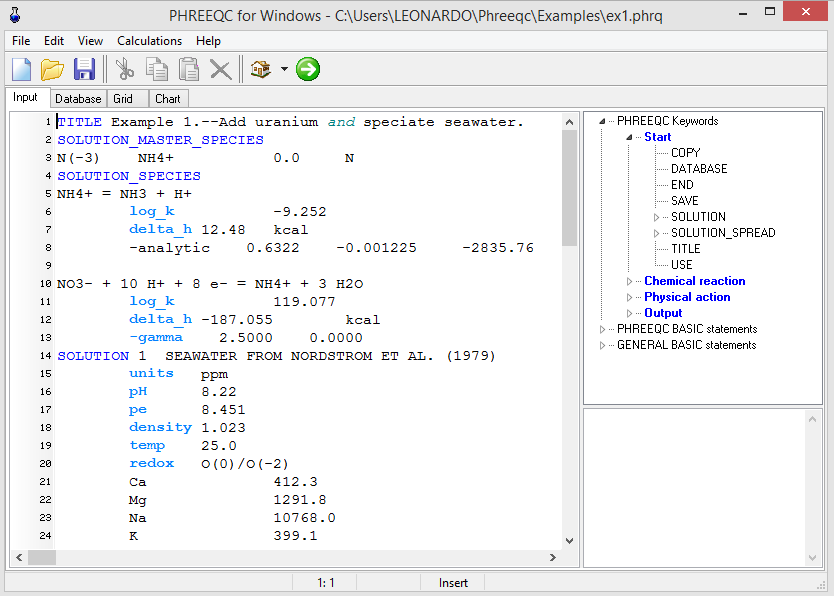
\includegraphics[width=100mm]{figures/pfw.png}
\caption{User interface of the PHREEQC for Windows (\emph{PfW})}
\label{fig:phreeqc-pfw}
\end{figure}

\begin{figure}[ht!]
\centering
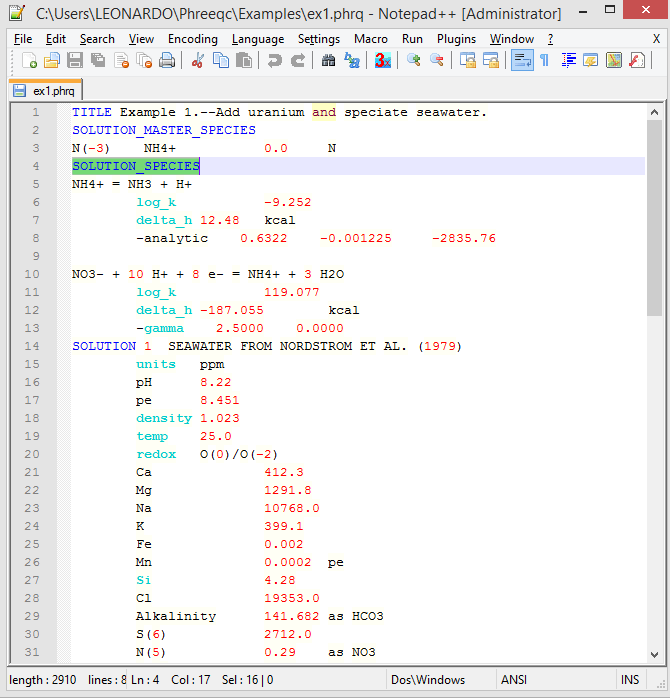
\includegraphics[width=100mm]{figures/notepad++Phreeqc.png}
\caption{Example of the PHREEQC Notepad++ plugin}
\label{fig:phreeqc-notepad++}
\end{figure}

\begin{figure}[ht!]
\centering
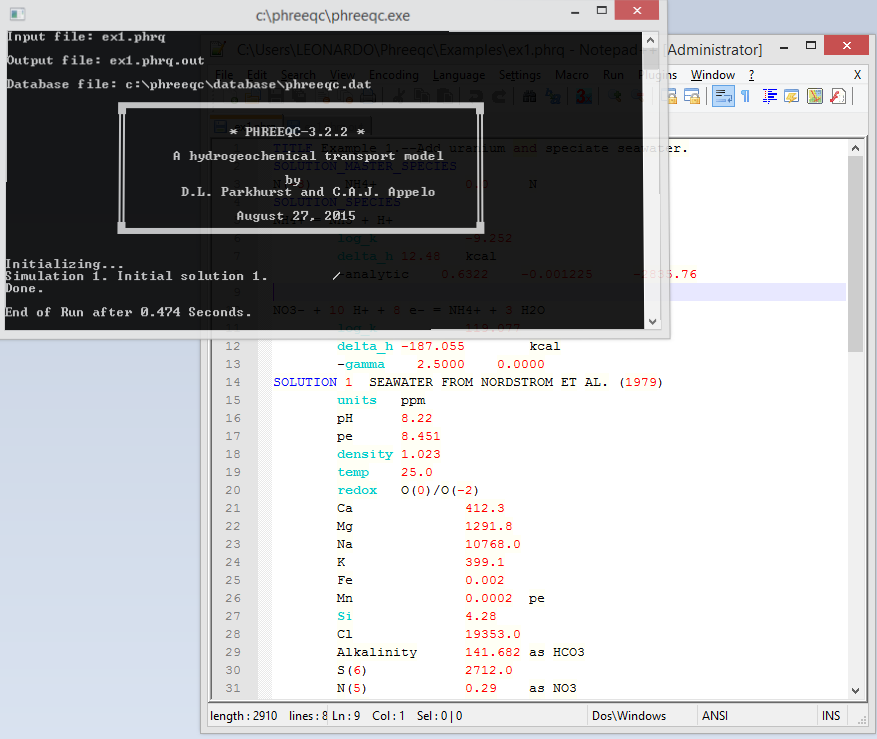
\includegraphics[width=100mm]{figures/notepad++PhreeqcProcess.png}
\caption{PHREEQC software called from the Notepad++ Plugin}
\label{fig:phreeqc-notepad++2}
\end{figure}

\begin{figure}[ht!]
\centering
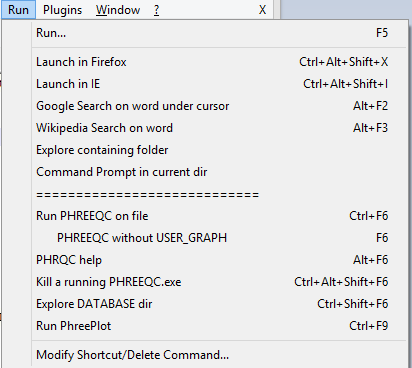
\includegraphics[width=100mm]{figures/notepad++run_menu.png}
\caption{PHREEQC software called from the Notepad++ Plugin}
\label{fig:phreeqc-notepad++3}
\end{figure}

\subsection{File formats}
All of the files discussed above are in the \emph{ASCII} text files format and, therefore, any regular text editor can be used. 
It is recommended that the editing of \emph{PHREEQC} files be done by using the NotPhreeqcce or notepad++ adapted version \cite{NotPhree:11}.

% IDEM - ACHO DESNECESSÁRIO
\subsection{Software Environment and Installation Procedures}
\emph{PHREEQC} has support for Windows (32 and 64-bit), MacOS (OS 10.6+) and Linux. \emph{PHREEQC} is currently on version 3 and with frequent updates, bug fixes and maintenance.

The \emph{PHREEQC} version for Windows has a self-extracting file that is available for download from the USGS website and easily installed. The \emph{UNIX} distribution comes with additional scripts and a makefile, and an instruction on how to compile and install the program.

%MINTEQ
\section{\emph{MINTEQ}}
\emph{MINTEQ} \cite{Felmy:84} is a geochemical program to model aqueous solutions and the interactions of aqueous solutions with hypothesized assemblages of solid phases. It has a particular inclination to calculate equilibrium composition of dilute aqueous solutions. The model is useful for calculating the equilibrium mass distribution among dissolved species, adsorbed species and multiple solid phases, although it has a much simpler treatment of the reactions. 

It was originally developed in FORTRAN77 by the \emph{Battelle Pacific Northwest Laboratory} (\emph{PNL}) and continues to be maintained by the \emph{Environmental Protection Agency} (\emph{EPA}) to perform the  necessary calculations regarding waste, sediments and ground water interaction. \emph{MINTEQ} does not consider the kinetic reactions and works at fixed temperature ($25$ degrees Celcius). 
An extensive database adequate to a broad range of problems is part of the software, and there is no need for the user to change nor add anything \cite{Brown:87} \cite{Allison:91}. The latest update on \emph{MINTEQ} dates from 1990, and since then, there has been only some improvements especially on the usability and calculations. This version was named \emph{MINTEQA2} and uses a well-developed thermodynamic database from the \emph{USGS}. During this review we will address the \emph{MINTEQA2} properties since it is the latest version and is clearly an improved version of the same program (\emph{MINTEQ}).

\subsection{Input/Output Options}
The input files for \emph{MINTEQA2} can be generated manually, but there is a supporting software called \emph{PRODEFA2} that guides the user to accomplish this task. \emph{PRODEFA2} is an interactive program used to create input files that will be addressed in details in section~\ref{minteq:interactions}. Four files compose the input of \emph{MINTEQA2}:
\begin{itemize}
\item Input file: The input file that contains the data input by the user. Typically, this file contains dissolved (i.e. Ca concentrations, pH, temperature) and solid phase (i.e. minerals, sorption sites) information for a water sample;
\item Database file: This file contains the thermodynamic constants that govern the processes of interest (i.e. complexation constants, mineral solubilities, activity constants) which will be used to conduct calculations;
\item Algorithm or executable file:  These files contain the algorithms of the code, which solve the specified problem (usually using an iterative numerical approach) within the constraints imposed by the Database files and the information in the Input file.
\item Output file: This file contains the results of the calculations performed by the Algorithm Files.
\end{itemize}

Among the input file's options, there are four levels of configuration. Each level controls some details of the simulation, and when these four levels are together, they compose a complete input file for \emph{MINTEQA2}. It is important to mention that if the user does not want to specify all the details, there are default options that enable any non-experienced user to execute simple simulations.
\begin{enumerate}
\item Displays the current settings of system parameters such as temperature as well as program flag settings such as the number of iterations allowed;
\item Specify the chemistry of the system;
\item This level works as a "line editor" in displaying by category or TYPE those species that have been explicitly entered through level 2;
\item Deals with utility functions (output file details, for example);
\end{enumerate}

If database, algorithm and output files are not specified, default options are used. Code ~\ref{minteqa2:input}  brings the \emph{MINTEQA2}'s input file used in the study case discussed in chapter~\ref{chapter:validation} and presented here as an example. The beginning of the file (first and second lines) contains a description of the simulation or input file; the third, fourth and fifth lines set configurations, such as temperature, unit chosen, eH, ionic strength, number of iterations, precipitation options. After that, the components that take part in the simulation, organized by internal id, concentration details and log of concentration are specified.

\begin{minipage}[c]{0.92\textwidth}
\begin{lstlisting}[frame=single, caption=\emph{MINTEQA2}'s input file, label=minteqa2:input]
LHDAMIANI - STUDY CASE
Comparative study           
25.00 MOLAL  0.000  0.00000E+00
0 0 1 0 1 0 0 0 1 1 0 0 0
0   0   0
    330  6.026E-09   -8.22 y                    /H+1               
    410  1.045E-02   -1.98 y                    /K+1               
    500  4.793E-01   -0.32 y                    /Na+1              
    150  1.053E-02   -1.98 y                    /Ca+2              
    460  5.439E-02   -1.26 y                    /Mg+2              
    732  2.889E-02   -1.54 y                    /SO4-2             
    180  5.595E-01   -0.25 y                    /Cl-1              

\end{lstlisting}
\end{minipage}



An excerpt of \emph{MINTEQA2}'s output is presented in Code ~\ref{minteqa2:output} - shows important parameters of the solution's components. The whole output file is divided into six parts:
\begin{enumerate}
\item Reproduction and interpretation of the input file;
\item Detailed listing of species read from the database files;
\item Iteration information and detailed information for each species;
\item Percentage distribution of components among dissolved and adsorbed species;
\item Provisional or equilibrated mass distribution, provisional or equilibrium ionic strength, equilibrium pH and pE, electrostatic surface potential and charge for electrostatic adsorption models;
\item Saturation indices for all database solids with respect to the solution;
\end{enumerate}


\begin{minipage}[c]{0.92\textwidth}
\begin{lstlisting}[frame=single, caption=\emph{MINTEQA2}'s excerpt from the output file, label=minteqa2:output]
...
_______________________________________________________________________
______________________________ PART 3 of OUTPUT FILE __________________
  MINTEQA2  v4.02   DATE OF CALCULATIONS:  5-JUN-2000  TIME: 14: 6:27



PARAMETERS OF THE COMPONENT MOST OUT OF BALANCE:

ITER      NAME       TOTAL mol/L   DIFF FXN   LOG ACTVTY    RESIDUAL
0   SO4-2           1.580E-03   6.594E-07    -2.91757    5.014E-07
1   SO4-2           1.580E-03   4.193E-04    -2.91775    4.192E-04
2   SO4-2           1.580E-03   8.125E-06    -3.01997    7.967E-06
3   SO4-2           1.580E-03   1.693E-07    -3.02220    1.135E-08

 ID No  Name        Total Conc(M)    Conc (M)  log Activity   Diff fxn
  410   K+1            7.700E-05     7.649E-05    -4.14759    5.093E-11
  732   SO4-2          1.580E-03     1.266E-03    -3.02224    3.557E-09
    2   H2O            0.000E+00    -1.049E-05    -0.00004    0.000E+00
  330   H+1            0.000E+00     3.398E-03    -2.50000    0.000E+00
  140   CO3-2          0.000E+00     2.916E-17   -16.66004    0.000E+00

-----------------------------------------------------------------------
...
\end{lstlisting}
\end{minipage}

\subsection{User Interaction}\label{minteq:interactions}
\emph{MINTEQA2} and \emph{PRODEFA2} interactions are completely independent programs and \emph{PRODEFA2} is used before \emph{MINTEQA2} in order to generate the input file that will be consumed by the latter. Everything is done through the command prompt, as explained below. \emph{PRODEFA2} provides a "walk-through" to generate an input file for \emph{MINTEQA2}.

After opening the software and providing a valid name, it asks which part of the input file the user wants to create or edit (Figure~\ref{minteq:init}). We will follow the suggested order and go through 4 levels, as previously discussed in this section. Figure~\ref{minteq:level0} shows the main menu, which shows the organization of all the levels and works as a central hub of information. Figure ~\ref{minteq:level1} displays the necessary information about level 1. To change any of the entries on this screen, the user must enter the number to the left of the entry and respond to the questions presented. All four levels carry out this type of interactions. Through these interactions, the user has access to the information in the database and can choose the data to be used for the model.

\begin{figure}[ht!]
\centering
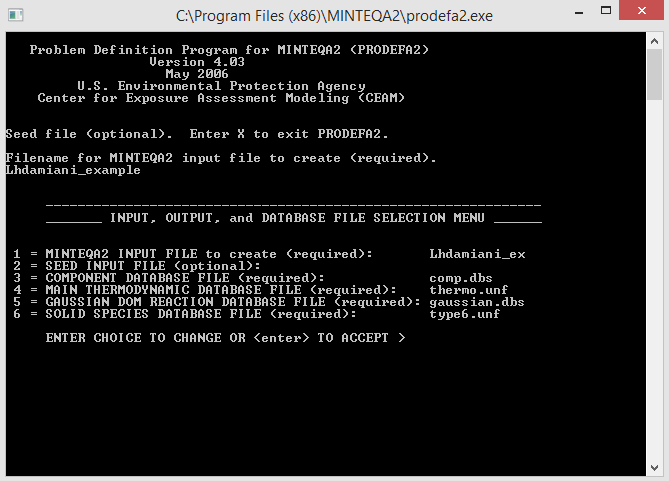
\includegraphics[width=100mm]{figures/minteq-init.png}
\caption{\emph{MINTEQA2} initial menu options}
\label{minteq:init}
\end{figure}

\begin{figure}[ht!]
\centering
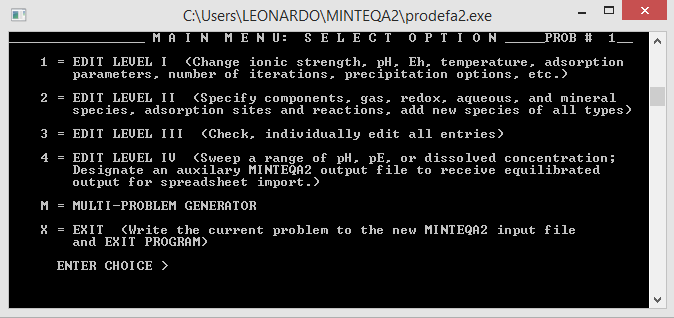
\includegraphics[width=100mm]{figures/minteq-level0.png}
\caption{\emph{MINTEQA2} main menu}
\label{minteq:level0}
\end{figure}

\begin{figure}[ht!]
\centering
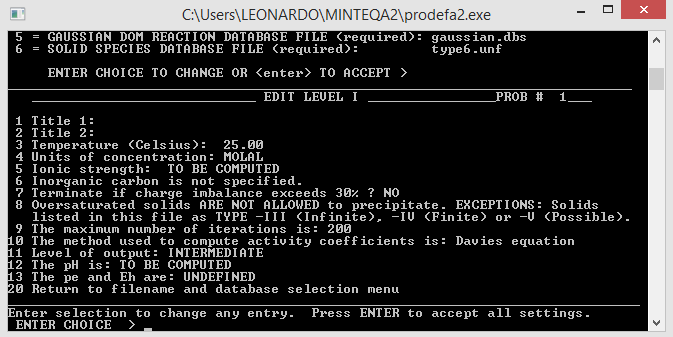
\includegraphics[width=100mm]{figures/minteq-level1.png}
\caption{\emph{MINTEQA2} Level 1 informations}
\label{minteq:level1}
\end{figure}


For example, we chose to add a specific aqueous species to show the \emph{PRODEFA2} interactions and present it step-by-step bellow:

\begin{enumerate}
\item Choose level 2 on main menu;
\item Choose option 1 (Specify AQUEOUS COMPONENTS: TOTAL CONCENTRATIONS or FIXED ACTIVITIES) inside the menu from level 2;
\item Choose option 1 (TOTAL DISSOLVED CONCENTRATION), it identifies how we want to entre this new component.
\item At this step, we are requested to enter the first letter for the component. Alternatives to this approach is to enter "-1" if you know the component id number or quit. We will add \ce{Na^+} to the system, and type the letter "N" and hit the enter button.
\item At this step, all the existing options available are shown. listed with an identifier. We are also requested to identify one of these to be added. This can be seen in ~\ref{minteq:Na+}.
\item After pressing \ce{Na^+}'s id (at this case was the number 4). We can finally enter the TOTAL DISSOLVED CONCENTRATION (MOLAL) of COMPONENT defined earlier on step 3. After adding the molal concentration for this species the system goes back to step 4 in case we want to continue adding other components.
\end{enumerate}

\begin{figure}[ht!]
\centering
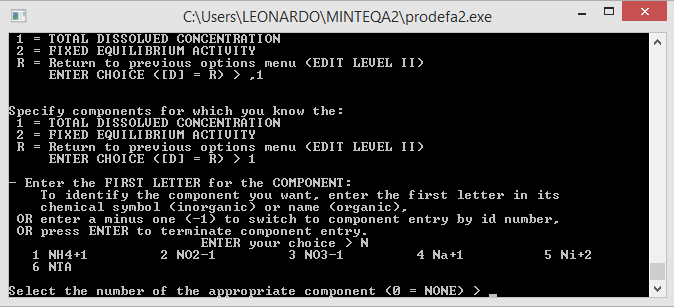
\includegraphics[width=100mm]{figures/minteq-Na+.png}
\caption{\emph{PRODEFA2}'s example of adding a specific aquoues species (\ce{Na+}) }
\label{minteq:Na+}
\end{figure}

There is also a software called \emph{Visual Minteq} that tries to "humanize" \emph{MINTEQ} and was maintained by the KTH Royal Institute of Technology, located in Stockholm, Sweden. The latest release date of \emph{Visual Minteq} latest is December 2013 at the version 3.0 and is available only for \emph{Windows} operating systems since it was developed in Visual Basic. 

\subsection{File formats}
All the files follow a regular text format (\emph{ASCII}) and their purpose is defined in the extension of the file. 
\begin{itemize}
\item Input files have the extension \emph{"INP"};
\item Test and help files have the extension \emph{"HLP"};
\item Output files have the extension \emph{"LST"};
\item Database files have the extension \emph{"DBS"} or \emph{"UNF"};
\item Input file have the extension \emph{"INP"};
\end{itemize}


% Juntei as duas partes como tu sugeriu.. deixei a parte de installation procedures .. qualquer coisa posso tirar depois se decidirmos nao utilizar.
\subsubsection{Software Environment and Installation Procedures}
It is currently at the version 4.03 (Windows only), and this release dates back to May 2006. The latest \emph{UNIX} distribution is version 3.12 (which was also called BETA for UNIX) and dates back to August 1996.
\emph{MINTEQA2} is easily installed by a self-extractor installer that can be downloaded from \emph{EPA}'s website \cite{minteq:website} and \cite{minteq:unix}. Included in the distribution package are also some important documentation, \emph{PRODEFA2} software and several input/output template files.
The UNIX version distribution comes with the source files and must be compiled and linked to run.

\section{\emph{SOLMINEQ.88}}
\emph{SOLMINEQ.88} is a geochemical modeling program written in FORTRAN 77 and based on SOLMNEQ \cite{Kharaka:73} with improved algorithms that resulted in a faster program execution and tighter convergence. The software has a database with the focus on organics aqueous species. It calculates the distribution of mass among aqueous species and complexes and calculates saturation indexes of minerals at different temperatures and pressures. It includes options as boiling, mixing of solutions, and partitioning of gases between water, oil and vapor phases. \emph{SOLMINEQ.88} also contemplates mass transfer with the effects of dissolution and precipitation of minerals and options to calculate activity coefficients \cite{Kharaka:88}. The original version has no UI, but there were further studies with the intention of creating a user-friendly program that can be used to generate, edit and analyze input and output files - \emph{SOLINPUT}.
\emph{SOLMINEQ.88} model has not been developed any further nor improved since its first release.

\subsection{Input/Output Options}
The input of \emph{SOLMINEQ.88} consists of two sets of data: fixed and variable. The first data contains the chemical composition of an aqueous fluid and options for processing these data; and the second data consists of the input required for using the first set of data.

The input file consists of six parts, and \emph{SOLINPUT} guides the user through all of them:
\begin{enumerate}
\item Basic Parameters: enter the chemical and physical data for that sample;
\item Flags: controls how the software interprets, processes, and displays the data;
\item pH: controls the details of how the pH calculation is done;
\item Mass transfer: defines which mass transfer capabilities are used;
\item User Log K: makes temporary changes and extensions to the database;
\item Additional ions and minerals: temporarily adds user defined ions and minerals to a particular simulation;
\end{enumerate}

The output file contains the results produced by \emph{SOLMINEQ.88}, and consists of six parts: An input data echo that shows the values and options selected for each sample; A table listing the calculated tolerance factor for successive iterations on the anions; A list of input to \emph{SOLMINEQ.88} including sample description, pH, Eh, temperature and so on; A table showing the distribution of species in solution; Ratios of a number of important cations and anions ; and the last one contains a table indicating the states of reactions for minerals considered:

\begin{minipage}[c]{0.92\textwidth}
\begin{lstlisting}[frame=single, caption=\emph{SOLMINEQ.88}'s excerpt from the output file, label=solmineq:output]
 : Test Sample #1 for SOLMINEQ.88 - Modified Seawater at 25 C
TEMP HI TEMP DENS PRESS
0.2500E+02 O.OOOOE+00 0.1023E+01 O.OOOOE+00
PH EHM EHMC EMFZSC
0.8200E+01 0.5000E+00 0.9000E+01 0.9000E+01
CONCENTRATION UNITS : PPM
Na K Li Ca
0.1077E+05 0.3991E+03 0.1810E+00 0.4123E+03
Si02 Cl S04 H2S
0.4280E+01 0.1935E+05 0.2712E+04 O.OOOOE+00
F P04 N03 NH3
0.1390E+01 0.6000E-01 0.2900E+00 0.3000E-01
Pb Zn Cu Mn
0.5000E-04 0.4900E-02 0.7000E-03 0.2000E-03
As U V
0.4000E-02 O.OOOOE+00 O.OOOOE+00
Acetate Oxalate Succinate CH4
0.1000E+00 0.1000E+00 0.1000E+00 0.1000E+00
\end{lstlisting}
\end{minipage}

\subsection{User Interaction}
The software that accompanies \emph{SOLMINEQ.88} and handles the generation of input files and all the interactions is named \emph{SOLINPUT} and described in \cite{Debraal:89}. All interactions are through command prompt input following displayed menus with several options. The user selects the option by entering the indication number and pressing enter (the indication number stays on the left of the option). Figure~\ref{solmineq:interaction} shows this example of interaction.

\begin{minipage}[c]{0.92\textwidth}
\begin{lstlisting}[frame=single, caption=\emph{SOLMINEQ.88}'s example of user interaction, label=solmineq:interaction]
	pH OPTIONS
1) Gas Addition Option
2) Gas-Water-Oil Distribution Option
3) Carbonate Mineral Saturation Option
4) C02 Option
5) Tolerance factor for Mineral and C02 Options
6) Return to Options Menu
Enter Choice (1-6)   __
\end{lstlisting}
\end{minipage}

\subsection{File formats}
All the files that \emph{SOLMINEQ.88} deals are regular \emph{ASCII} text files and any text editor can be used to create, edit or view the files. The database files from \emph{SOLMINEQ.88} have the extension "TBL", while the input and output files, "IN" and "OUT", respectively. 
Some optional file with the extension "MIXFLE" can be used to specify mixture properties. Finally, if the user activates the restart option, also known as pickup option, the file "OUTIN" will be generated and it contains data from the current run.

\subsection{Software Environment and Installation Procedures}
As mentioned, \emph{SOLMINEQ.88} had only one release and has been discontinued since then. It is available only for the \emph{Windows} operating system.

\emph{SOLMINEQ.88} distribution requires knowledge of compiling and linking \emph{FORTRAN77} programs. It also comes with the software \emph{SOLINPUT}.

%GEOCHEMICAL SPECIATION ANALYSIS
\section{Discussion}
In this section some important aspects and issues of each one of the software presented earlier are compared, analyzed, and discussed. Regarding geochemical features, table~\ref{tab:comparativeTable} brings certain aspects and features of the software.

\begin{table}
\caption{Geochemical comparison between speciation softwares}
\label{tab:comparativeTable}
\centering
\begin{tabular}{r|cccccccc}
SOFTWARE &
\rot{Aqueous Complexation} &
\rot{Precipitation and Dissolution Mass Balancing} & 
\rot{Reaction path} &
\rot{Kinetics} &
\rot{Multi-Activity Coefficient methods} 
    \\ \hline
EQ3/6        	&  \OK &  \OK & \OK & \OK & \OK    \\ 
PHREEQC        &  \OK &  \OK  & \OK & \OK &  \\
MINTEQA2        &  \OK  &  \OK & & &    \\ 
SOLMINEQ.88	& \OK& \OK&\OK & \OK & \OK\\
\hline
\end{tabular}
\end{table}

From the perspective of computer science, we analysed and evaluated the software for the software engineering aspect taking into account all of the features described and extensively discussed in chapter ~\ref{chapter:basic}.

Following points were taken into consideration:
\begin{itemize}
\item The costs: Costs are probably the most important thing that people look first when choosing software; however, it should not be the deciding factor. Different solutions use different pricing models and according to the purpose and utilization of the software.

\item Setup and versioning: The installation of software is the act of making it ready for execution. Depending on the software different options are used to copy/generate files from the installation files to the local computer to be accessed by the operating system (\emph{OS}). The \emph{OS} also influences how this process is done. Each software has a different distribution package for different \emph{OS}. Commonly software are distributed only to specific \emph{OS}. Also common are software with disparate versions according to the \emph{OS}, resulting in divergent features available on the same software defined by the \emph{OS} types.

\item Customization and Integration: Is the software a standard solution, and its supplier interested in making changes? This is the typical scenario where the user has great chances of finding problems ahead. Therefore, an interesting exercise is to think of how this software communicates with others. Options like  ``import'' and ``export'' are vital when working with a large amount of data. With the advances in software, different software can be used to analyse the output and to be able to reach deeper insights about the information available. 

\item Security and Control: Security is one of the main issues one faces when considering a software. Data privacy is an important criteria. Ensuring that the software can guarantee no data loss or data leakage is important. The solutions that provide direct control to the database, details, and processes are most likely to require data privacy.

\item Infrastructure: When choosing a software, the infrastructure it requires need to be carefully analyzed. Does it require Internet access? How much space on disk and memory does it use? Extra costs may be incurred if this is not addressed.

\item Core functionality: This is one of the most important points to be analyzed. How good is the software focus on the needs of the user, and how good is the value the software brings to its users?

\item Graphical User Interface (\emph{GUI}) and visualization: This feature handles the interaction between the users and the software. When the software has a complex domain, such as geochemical modeling, the \emph{GUI} is even more important. It is responsible for allowing the user to consider all necessary possible options. The perfect \emph{GUI} takes into consideration the necessary human behavior, senses, and how we interact with our world (from electronic devices to human relationships).

\item Support and Maintenance: If the software, for some unknown reason, goes down, is the user able to reach someone for troubleshooting? Will the user be able to find a users' community to debate and share knowledge? If the software has a support team working to fix bugs, improve the performance, add new features and sharpen some of the old features, it means that the user will have a better infrastructure to work with.

\item Database: All the data manipulated inside a software is stored and organized in a database. There are multiple ways of doing this. Many important things must be taken into account to decide which database fits best to the software. Since the 80's the relational database model represented by the \emph{SQL} language has been the most popular. A conceptual database model is strongly recommended to produce a schema that considers all the structure and information needed by this software. Along the database schema, the security of this database must be addressed properly, for consistency and privacy. A good database design avoids redundant data (unnecessarily duplicated data). Poorly designed database generates inconsistent data (inaccurate data), which will lead to wrong decisions and, therefore, can result in failure of the software.
\end{itemize}


\subsection{Existing Thermodynamic datasets}
The contents of the databases are extracted from the \emph{Lawrence Livermore National Laboratory (LLNL)} thermodynamic datasets that are used in \emph{EQ3/6}, \emph{PHREEQC} and others. The data sets are contributions from many authors that had measured thermodynamical and kinetic parameters of the minerals and reactions minerals over the years. The following is a small excerpt that illustrates the structure that the information is organized in the \emph{LLNL}'s flat file:

\begin{itemize}
\item Parameters: Many used parameters are stablished on this section, among them are temperatures, pressures, debye huckel coefficients, bdot coefficients...
\begin{lstlisting}[frame=single, caption=Excerpt of the section Parameters]
* temperatures
         0.0000   25.0000   60.0000  100.0000
       150.0000  200.0000  250.0000  300.0000
* pressures
         1.0134    1.0134    1.0134    1.0134
         4.7600   15.5490   39.7760   85.9270
\end{lstlisting}
\item Elements: This section is composed of information on pure elements. It also lists the mole weights of elements and the abreviation: 
\begin{lstlisting}[frame=single, caption=Excerpt of the section Elements]
Oxygen          (O )          mole wt.=   15.9994
Silver          (Ag)          mole wt.=  107.8680
Aluminum        (Al)          mole wt.=   26.9815
\end{lstlisting}
\item Basic Species: This section lists atomic or molecular structural units for a mineral:
\begin{lstlisting}[frame=single, caption=Excerpt of the section Basic Species]
H2O
     charge=  0.0      ion size=  0.0 A      mole wt.=   18.0152
     2 elements in species
       1.000 O               2.000 H
\end{lstlisting}


\item Redox Couples: This sections includes all chemical reactions in which molecules have their oxidation states changed. 
Redox reactions involve the transfer of electrons between species.
The name comes from two concepts involved with electron transfer (reduction - loss of electrons - and oxidation - gain of electrons). Example:

\begin{minipage}[c]{0.92\textwidth}
\begin{lstlisting}[frame=single, caption=Excerpt of the section Redox Couples]
Cr++
     charge=  2.0      ion size=  5.0 A      mole wt.=   51.9960 g
     4 species in reaction
      -1.000 H+              0.500 H2O             1.000 Cr+++
      -0.250 O2(aq)
        33.6814   29.9291   25.6126   21.6721
        17.7896   14.7267   12.2289   10.1676
\end{lstlisting}
\end{minipage}


\item Aqueous Species: This sections contains the water solutions. The word aqueous is applied to a solution or mixture in which water is the solvent. When a chemical species has been dissolved in water, this is denoted by writing (aq) after the chemical name. Example:

\begin{minipage}[c]{0.92\textwidth}
\begin{lstlisting}[frame=single, caption=Excerpt of the section Aqueous Species]
CO2(aq)
     charge=  0.0      ion size=  4.0 A      mole wt.=   44.0098 g
     3 species in reaction
      -1.000 H2O             1.000 H+              1.000 HCO3-
        -6.5570   -6.3660   -6.3325   -6.4330
        -6.7420   -7.1880   -7.7630   -8.4650
\end{lstlisting}
\end{minipage}

\item Minerals: This sections lists the physical properties and chemical formula of minerals: 

\begin{minipage}[c]{0.92\textwidth}
\begin{lstlisting}[frame=single, caption=Excerpt of the section Minerals]
Calcite                         type= carbonate
     formula= CaCO3
     mole vol.=   36.934 cc      mole wt.=  100.0892 g
     3 species in reaction
       1.000 Ca++            1.000 HCO3-          -1.000 H+
         2.0683    1.7130    1.2133    0.6871
         0.0762   -0.5349   -1.2301   -2.2107
\end{lstlisting}
\end{minipage}

\item Gases: This section lists individual atoms (e.g. noble gases or atomic gases), elemental molecules made from one type of atom (e.g. oxygen), or compounds made up of two or more molecules (e.g. carbon dioxide). Example: 

\begin{minipage}[c]{0.92\textwidth}
\begin{lstlisting}[frame=single, caption=Excerpt of the section Gases]
CO2(g)
     mole wt.=   44.0098 g
     3 species in reaction
      -1.000 H2O             1.000 H+              1.000 HCO3-
        -7.6827   -7.8184   -8.0628   -8.3849
        -8.8297   -9.3208   -9.8841  -10.6132
\end{lstlisting}
\end{minipage}

\item Oxides: This sections contains the chemical compounds that consists of at least one oxygen atom and one other element in its chemical formula, and also does not include silica (Si): 

\begin{minipage}[c]{0.92\textwidth}
\begin{lstlisting}[frame=single, caption=Excerpt of the section Oxides]
Al2O3
     mole wt.=  101.9616 g
     3 species in reaction
      -6.000 H+              2.000 Al+++           3.000 H2O
\end{lstlisting}
\end{minipage}
\end{itemize}


To achieve an applicable comparison we give grades from 1 to 5 to each aspect (where 1 is the lowest and 5 the highest possible grade). This "grading system" is done with the intention of comparing and normalizing the attributes of the software (see table ~\ref{tab:comparativeSoftwareTable}\footnote{Source:Author}).

\begin{table}
\caption{Qualitative analysis of the Geochemical Speciation Softwares}
\label{tab:comparativeSoftwareTable}
\centering
\begin{tabular}{r|ccccccccc|ccc}

SOFTWARE &
\rot{Costs} &
\rot{Setup and versioning} & 
\rot{Customization and Integration} &
\rot{Security and Control} &
\rot{Infrastructure} &
\rot{Core functionality} &
\rot{Graphical User Interface} &
\rot{Support and Maintenance} &
\rot{Database}  &
\rot{Overall Average} 
    \\ \hline
EQ3/6        	& 2 & 2 & 1 & 1 & 3 & 5 & 1 & 1 & 1 & 1.88 \\ 
PHREEQC         & 4 & 4 & 2 & 2 & 3 & 4 & 2 & 3 & 1 & 2.77 \\ 
MINTEQA2        & 4 & 2 & 1 & 1 & 2 & 2 & 1 & 1 & 1 & 1.66\\ 
SOLMINEQ.88	    & 3 & 1 & 1 & 1 & 1 & 5 & 1 & 1 & 1 & 1.66\\ 
\hline
\end{tabular}
\end{table}


\newpage

%SUMMARY
\section{Summary}
\begin{itemize}
\item EQ3/6: It represents a landmark in Geochemical Modeling. Unfortunately, it is inaccessible due to the elevated cost of licensing. The vast amount of information available online about \emph{EQ3/6} makes it an excellent source of information.  It used the computing tools and options that were available in 1970’s and 80’s, until the latest known release date in 1992. Since then, computing has clearly evolved, making it an obsolete and difficult to use. It has a large database with many pieces of information, but the contents are not transparent. It is hard to understand what exactly is the software doing; verifying if that is what the users wants is even more difficult. It is also important to mention that in \emph{EQ3/6}  documentation it recommends the user to use operating system commands (i.e. \emph{ctrl+c}) to interact with the software - which is a highly risky procedure in modern computers.

\item PHREEQC: It is the best option for users not experienced with software. It has a \emph{GUI} and comes with a self-extractor installer. Important to mention here is that \emph{PHREEQC}'s \emph{GUI} is far from what a typical user of current era might expect. It is not clear in many aspects, and its usability is far from regular. In the geochemical modeling area, not all the users are familiar with tasks as compiling and linking computer programs. \emph{PHREEQC} allows anyone with an interest to have a chance to perform a geochemical modeling simulation, even as many people have different ways of defining the problem. Database in \emph{PHREEQC} seems to be a problem, as it uses a flat file database.

\item MINTEQA2: From the geochemical point of view, \emph{MINTEQA2} is the simpler of the four software analyzed in this work. The user interaction can be painful for anyone who are not familiar with command prompts. The complexity of the input file also makes it difficult to use. Creating an input file without the subsidiary software \emph{PRODEFA2} is a task close to impossible and learning how to use this subsidiary software is a very costly task. Taking into account that its last release dates back to 2006, it is difficult to justify using \emph{MINTEQA2}.

\item SOLMINEQ.88: This is another software that was a pioneer and laid the groundwork for many others to improve and progress the knowledge of geochemical modeling. \emph{SOLMINEQ} used the computing tools that were accessible when it was developed in 1980’s. There are less costly options easily attainable today, thus it is no longer a popular option for geochemical modeling.


\end{itemize}
\newpage
%%%%%%%%%%%%%%%%%%%
%                                                        %
% SHPECK - SPECIATION MODEL  %
%                                                        %
%%%%%%%%%%%%%%%%%%%


\chapter{\emph{SHPECK} - Speciation Model}
\label{chapter:SHPECK}

\emph{SHPECK} is a equation-based simulator, there is a governing theory that can guide the construction of mathematical models based on a set of equations. The “equation-based” term refers to simulations based on the kinds of global equations we associate with physical theories - many of these theories present in the foundation concepts of \emph{SHPECK} originally from the \emph{Phase Rule}. Phase rule allows us to predict the number of stable phases that may exist in equilibrium for a particular system and is describe fully in \cite{Garrels:65} and is the base principle used in chemical speciation.

As a computer simulation software, \emph{SHPECK} represents the entire process. This process includes choosing a model; finding a way of implementing that model in a form that a computer can run; calculating the output of the algorithm; visualizing and studying the resultant data.

This chapter will guide through all the aspects of the development of \emph{SHPECK} - a geochemical speciation modelling software. 

\section{Specification}
\emph{SHPECK} is a geochemical speciation modelling software responsible for calculating the distribution of dissolved species between free ions and aqueous complexes and also saturation indexes for different minerals. 

\section{Architecture}
The architecture of a software is responsible for assuring that all the internal and external stakeholders' concerns are preserved, addressed and satisfied. To not develop something that will not need restructuration and code refactoring later, it is necessary to see the big picture of the whole \emph{SHPECK}'s project. This will drive and be present during the entire development, starting with the technical decisions until the satisfaction of the final user.

Figure ~\ref{fig:shpeck-architecture} brings the software architecture of \emph{SHPECK}, which is modelled following the popular concept of \emph{Model-View-Controller} (MVC) \cite{Gamma:94}. \emph{MVC} is an architectural pattern that divides the software into three interconnected parts:
\begin{itemize}
\item Model: It is an object representing data or even activity. For example, the algorithm and math behind calculating the activity coefficient by Debye-Huckels' formula.
\item View: It is some form of visualization of the state of the model. For example, which are the solutes that the user wants to add into the simulation?
\item Controller: It offers facilities to change the state of the model. For example, define which algorithm for calculating the activity coefficient according to the user's choice or the value of the ionic strength (if the user did not specify which one to use).
\end{itemize}

\begin{figure}[ht!]
\centering
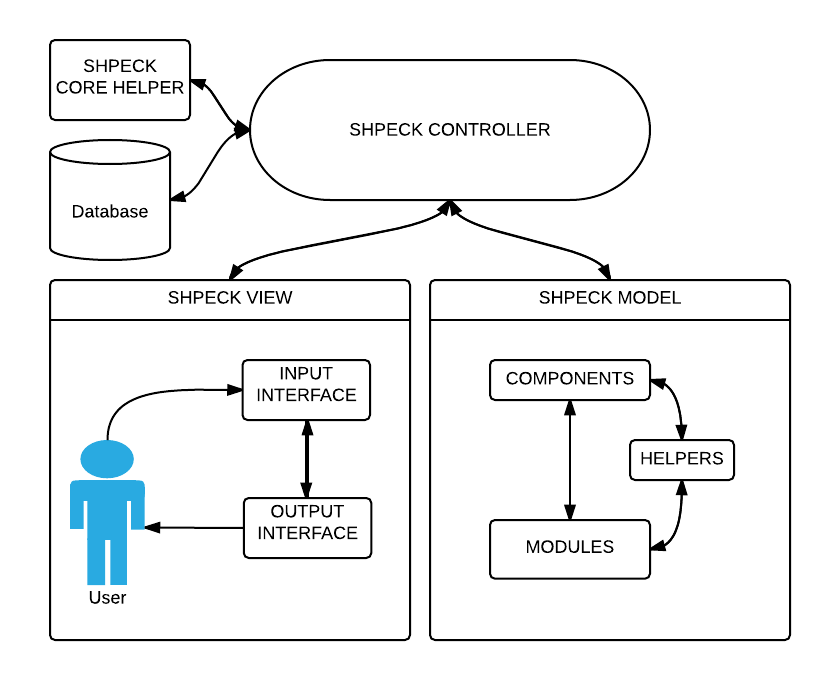
\includegraphics[width=100mm]{figures/shpeck-architecture.png}
\caption{Architecture of the \emph{SHPECK} software}
\label{fig:shpeck-architecture}
\end{figure}

\subsection{Technical Specification}
\emph{SHPECK} is a software developed using C++, which is a general-purpose programming language. C++ has a bias towards system programming that supports efficient low-level computation, data abstraction, object-oriented programming, and generic programming \cite{Dale:04} \cite{Stroustrup:97}. It provides powerful and flexible mechanisms for abstraction; that is, language constructs that allow the programmer to introduce and use new types of objects that match the concepts of an application needed. Thus, C++ supports styles of programming that rely on relatively direct manipulation of hardware resources to deliver a high degree of efficiency. It can also address higher-level styles of programming that rely on user-defined types to provide a model of computation that is closer to human's view of the task being performed by a computer. Application libraries often support these higher level styles of programming. While developing Shpeck, two supporter tools were adopted:
\begin{itemize}
\item \emph{Qt} : It is a cross-platform application and UI framework for developers using C++  \cite{Qt:14}. \emph{Qt} turns the development fast and easy, with lots of inbuilt library classes it provides a comprehensive range of functionality which also turns the debugging and testing way more productive and effective.
\item \emph{Armadillo} : It Is a C++ linear algebra library that provides classes for vectors, matrices, cubes and a whole set of functions to operate on the classes \cite{arma:14}. With a syntax similar to Matlab and an up-to-date support with upgrades and new releases almost every month.
\end{itemize}
Important to mention that the system is being developed using \emph{MAC} but the whole development process always took into account the goal to develop a multi-platform software to be distributed either in \emph{Windows, UNIX} and \emph{MAC}.

\section{Governing equations}
%These chemical equations are a mathematical model that drives all the methods that are executed in \emph{SHPECK}, its behavior defines all the steps and in which order they are presented. This set of equations models a real-world system and is named \emph{computer simulation model}.

\emph{SHPECK} uses the thermodynamic equilibrium reaction as equations for the calculation of multiphase systems in equilibrium, the details of these reactions are discussed in details in chapter ~\ref{chapter:basic}. A set of mass-action equations (as in equation ~\ref{eq:massaction}) compose the system; The number of species and compounds that coexist in the system define the number of equations. These equations model the geochemical speciation closed system and take into account all the chemical properties.

Aside with the mass-action equations we must have other constraints to solve the equilibrium state of the system. In \emph{SHPECK}, we use the concentration of the species (other possible constraints are the solute activity, the number of moles, total volume, etc.) to deal with the equilibrium state of the system.
This configuration generates a system where there are \emph{U} unknowns, {M} mass-action equations and \emph{E} equilibrium constraints. 
\begin{equation}\label{equilibrium_reaction}
U = E + M
\end{equation}
The unknowns values represents the number of moles of each specie in the system.

\section{Numerical Method}
In order to solve the system composed of the equilibrium state of the mass-action equations and the equilibrium constraints, \emph{SHPECK} uses a numerical methodology that computes simultaneously and find the value of the unknowns.


The numerical method applied a modification of the \emph{Newton's method} (also known as Newton-Raphson method), which is a method for finding successively better approximations to the roots of a set of equations. It works with a derivative approach to the equations, which optimizes the time consumed to find the roots and makes the representation of the system easier.

\emph{SHPECK} uses the \emph{Gauss-Newton}'s method to solve a nonlinear system of equations which results in finding the roots of continuously differentiable equations. 

The \emph{Gauss-Newton}'s method is applied in order to achieve the best approximation possible to the solution that is being sought. It since it is an iterative algorithm where each step consists in minimizing the first-order approximation of the solution. \emph{Gauss-Newton}'s method is a modification of \emph{Newton}'s method (also known as \emph{Newton-Raphson}'s method) for finding a minimum of a function. Its difference from regular \emph{Newton}'s method is that second derivatives are not required. \emph{Gauss-Newton}'s method is used to solve a system of coupled nonlinear equations. The first-order approximation of the function starts with an initial guess for the minimum values, the method proceeds by the iterations as shown in equations ~\ref{eq:gaussNewtonMethodEq1} and ~\ref{eq:gaussNewtonMethodEq2}.

\begin{equation}
\label{eq:gaussNewtonMethodEq1}
F(x+1) = F(x) - J^{-1} * R
\end{equation}

or 

\begin{equation}
\label{eq:gaussNewtonMethodEq2}
F(x+1) = F(x) - \frac{F(x)}{F'(x)}
\end{equation}

Where $F$ is function's result for the applied $x$, $J^{-1}$ is the inverse of the Jacobian matrix, and $R$ is the residual matrix \cite{Isaacson:66}.

The $R$ residual vector is defined as a vector containing the resulting values for each equation.

\begin{equation}
\label{eq:residualVector}
R = \begin{pmatrix}
 F(x_1) \\
 \vdots \\
 F(x_m)
 \end{pmatrix}
\end{equation}

Where $m$ is the number of unknowns (or mass-action equations plus equilibrium constraints).


The algorithm consists of iteratively calculating new approximations for the unknown values, through the matrix equation:

\begin{equation}
\label{eq:iterativelyAlgorithm}
[J]^{-1}_{iteration}* \alpha [U]_{iteration+1} = [R]_{iteration}
\end{equation}

Where $J$ is the Jacobian Matrix; $ \alpha [U]_{iteration+1} $ is the unknown composition at the next iteration; iteration is the iteration number and $R$ is the residual matrix. With this, is possible to state the $[U]_{iteration+1}$ value with:

\begin{equation}
\label{eq:CompositionCalculation}
[U]_{iteration+1} = [U]_{iteration} + \alpha [U]_{iteration+1}
\end{equation}


The initial guess of the solutions is an approximation that the user provides to the \emph{Gauss-Newton}'s method. This method needs a \emph{seed} to start the calculations (usually this guess is used for $F(0)$). 
If the guess is close to the real root value than the number of iterations necessary to obtain the solution will be small. If the guess is something completely nonsense, and far from the real solution, more iterations are going to be needed to find the correct solution.

The \emph{Jacobian Matrix} receives the equations and generates a model that does it automatically The \emph{Jacobian Matrix} is the matrix of all first-order partial derivatives of the equation and it is defined as

\begin{equation}
\label{eq:JacobianDefinition}
J_{mn} = \frac{\partial y^m}{\partial x^n}
\end{equation}

where the $y^i$'s are a new coordinate system defined in terms of the original coordinate system, the $x^i$'s. In differential equation theory, the Jacobian matrix plays a key role in defining the stability of solutions.

Specifically, \emph{SHPECK}'s equations can be described as: $F_1(x_1,..., x_n)$,...,$F_m(x_1,...,x_n)$. The partial derivatives of all these equations with respect to the variables $x_1,...,x_n$ can be organized in a m-by-n matrix, the Jacobian matrix, as bellow:

\begin{equation} 
J =
 \begin{pmatrix}
  \frac{\partial F_1}{\partial x_1} & \cdots & \frac{\partial F_1}{\partial x_n} \\
  \vdots  & \ddots & \vdots  \\
  \frac{\partial F_m}{\partial x_1} & \cdots &   \frac{\partial F_m}{\partial x_n}
 \end{pmatrix}
\end{equation}

In our case, $m = n$ and the \emph{jacobian matrix} is a square matrix and is generated once. With all the equations selected and organized, the derivatives of each reaction towards each variable are calculated and the \emph{jacobian matrix} is modeled and stored. 

Important to realize that the main complication with using a the \emph{Gauss-Newton}'s method to solve a system of nonlinear equations is defining all the functions included in the \emph{Jacobian Matrix}. As the number of equations and unknowns increases (n), so does the number of elements in the \emph{Jacobian} ($n^2$).

\section{Algorithm}

\emph{SHPECK}'s algorithm takes as its input a specification of the system's state. For example, the values for the concentrations of the species in the solution, the temperature of the system, the method to calculate activity coefficient, etc. It then calculates the system's state by executing all the processes in the necessary order that the model was conceptualized. 
Figure ~\ref{fig:Shpeck-algo} presents the high-level algorithm in details; is important to understand that each of the boxes in this algorithm represents a set of instructions, calculations and conditional clauses. Due to this work's scope we only specify the algorithm inside the box called "Newton's Method Solver", understanding how the governing equations controls the numerical methods is a fundamental piece. Newton's Method Solver internal algorithm is presented in figure ~\ref{fig:Shpeck-algo-newton}. 
\begin{figure}[ht!]
\centering
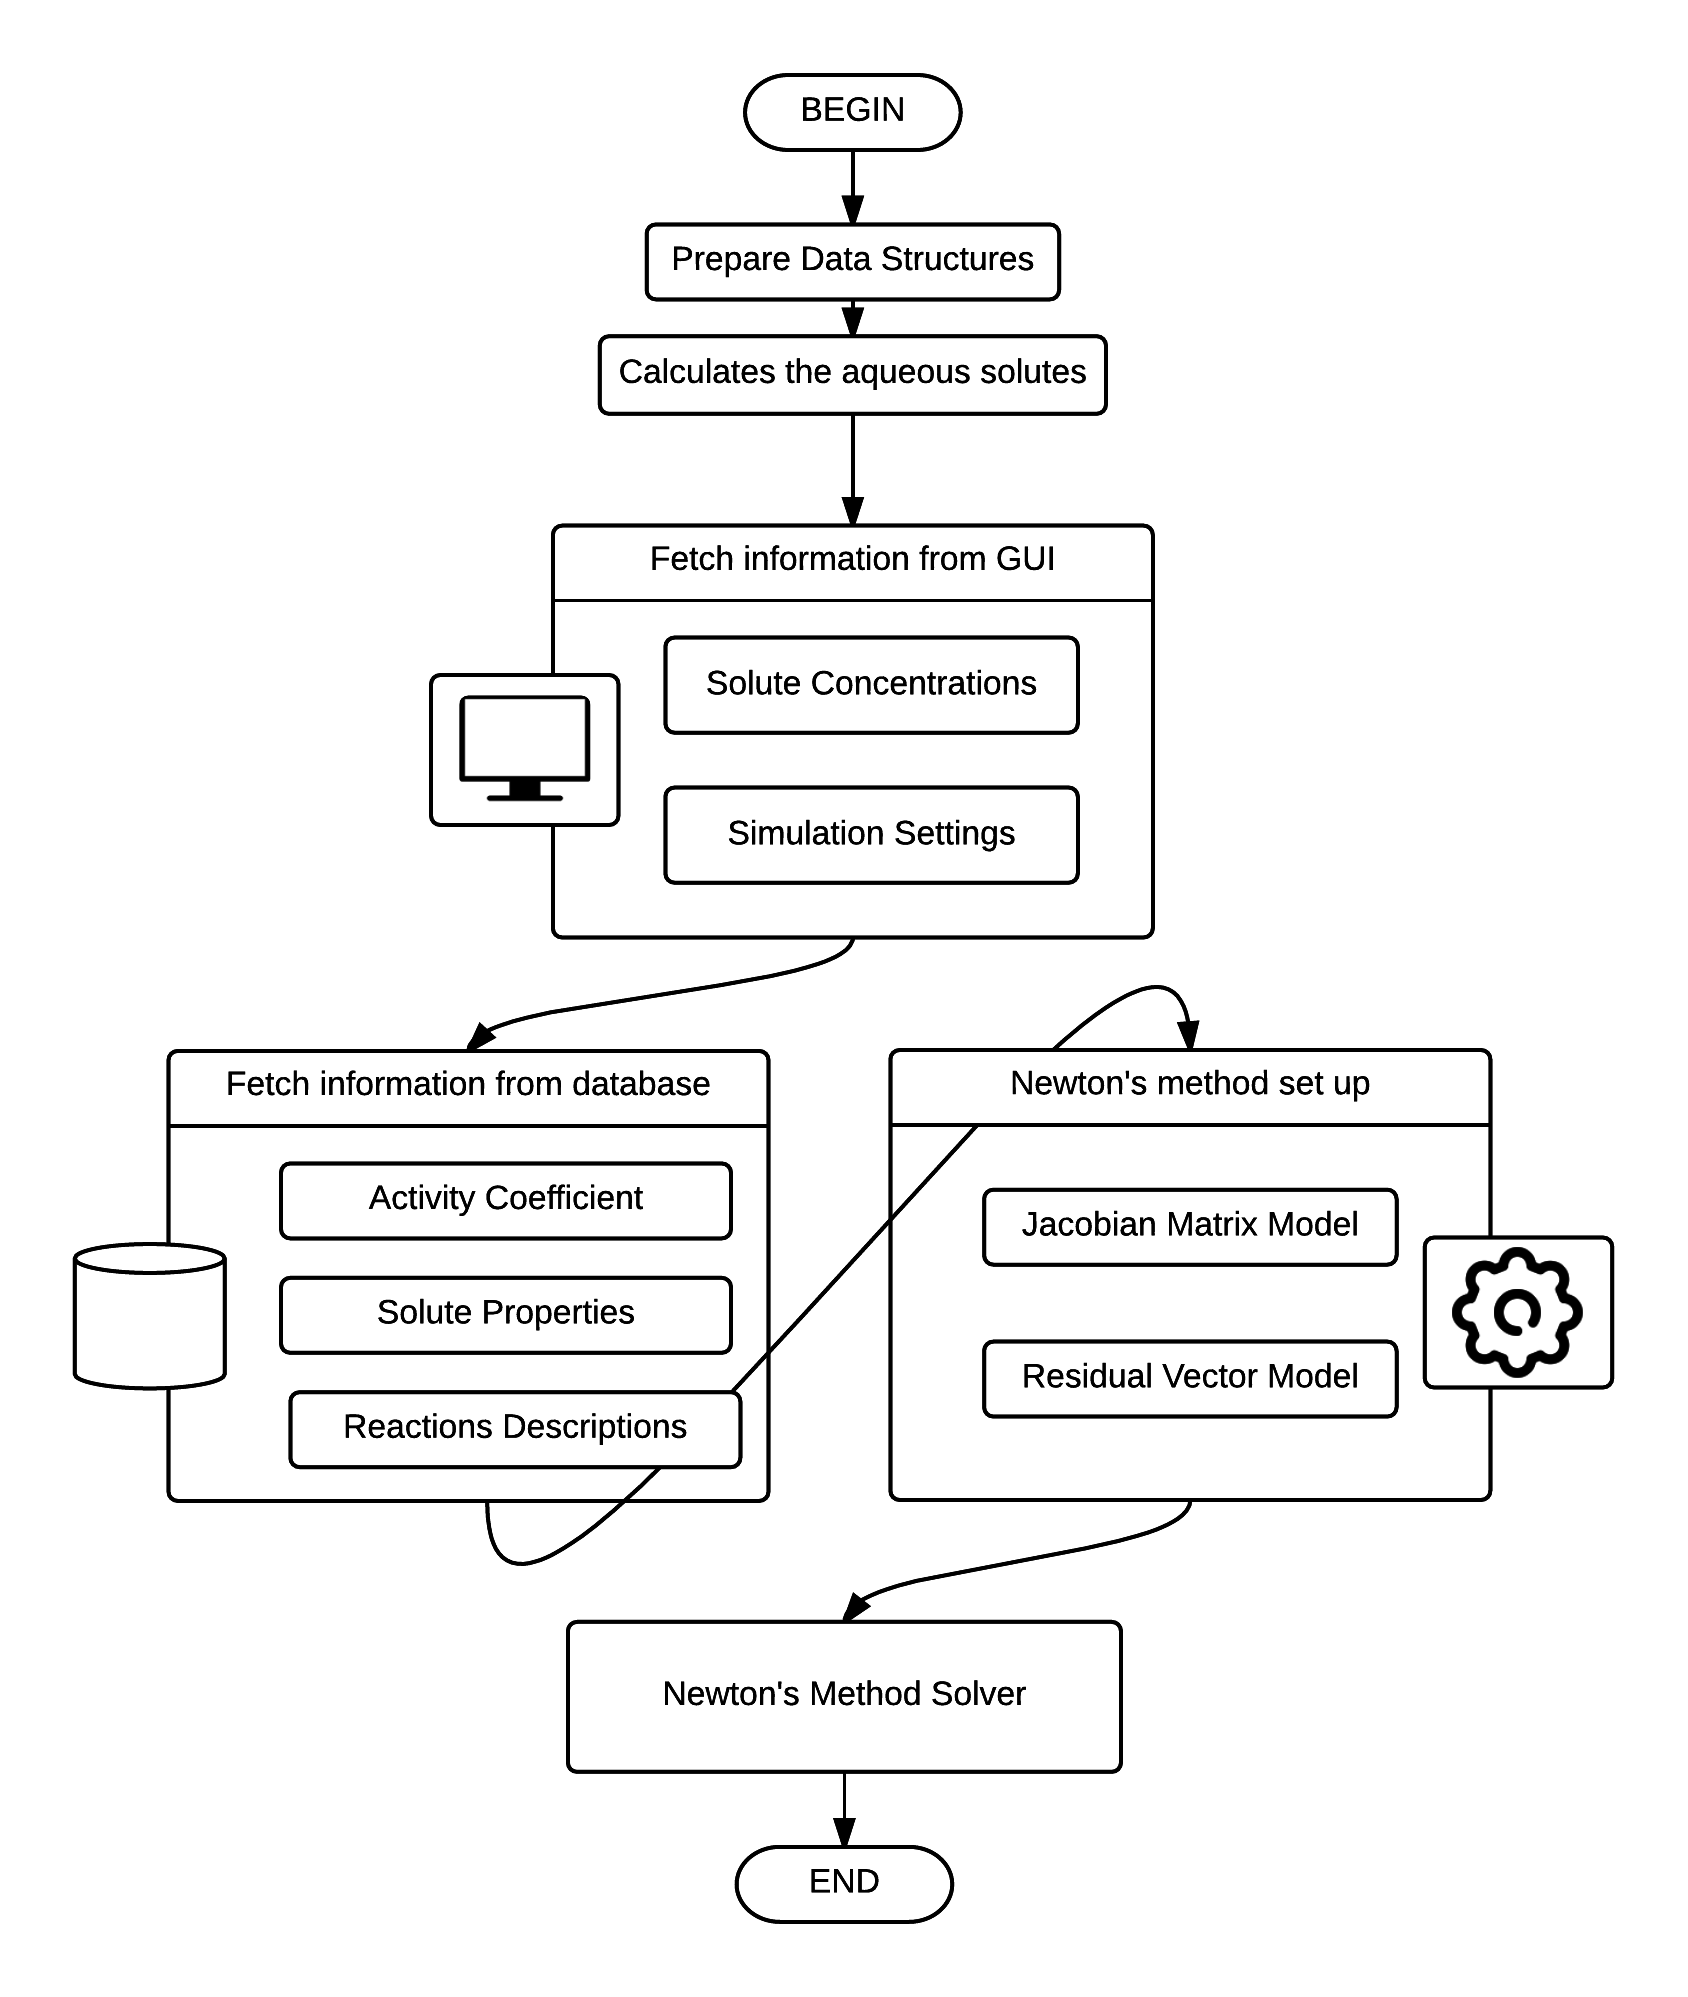
\includegraphics[width=100mm]{figures/Shpeck_algo3.png}
\caption{High-level algorithm of \emph{SHPECK}}
\label{fig:Shpeck-algo}
\end{figure}
\begin{figure}[ht!]
\centering
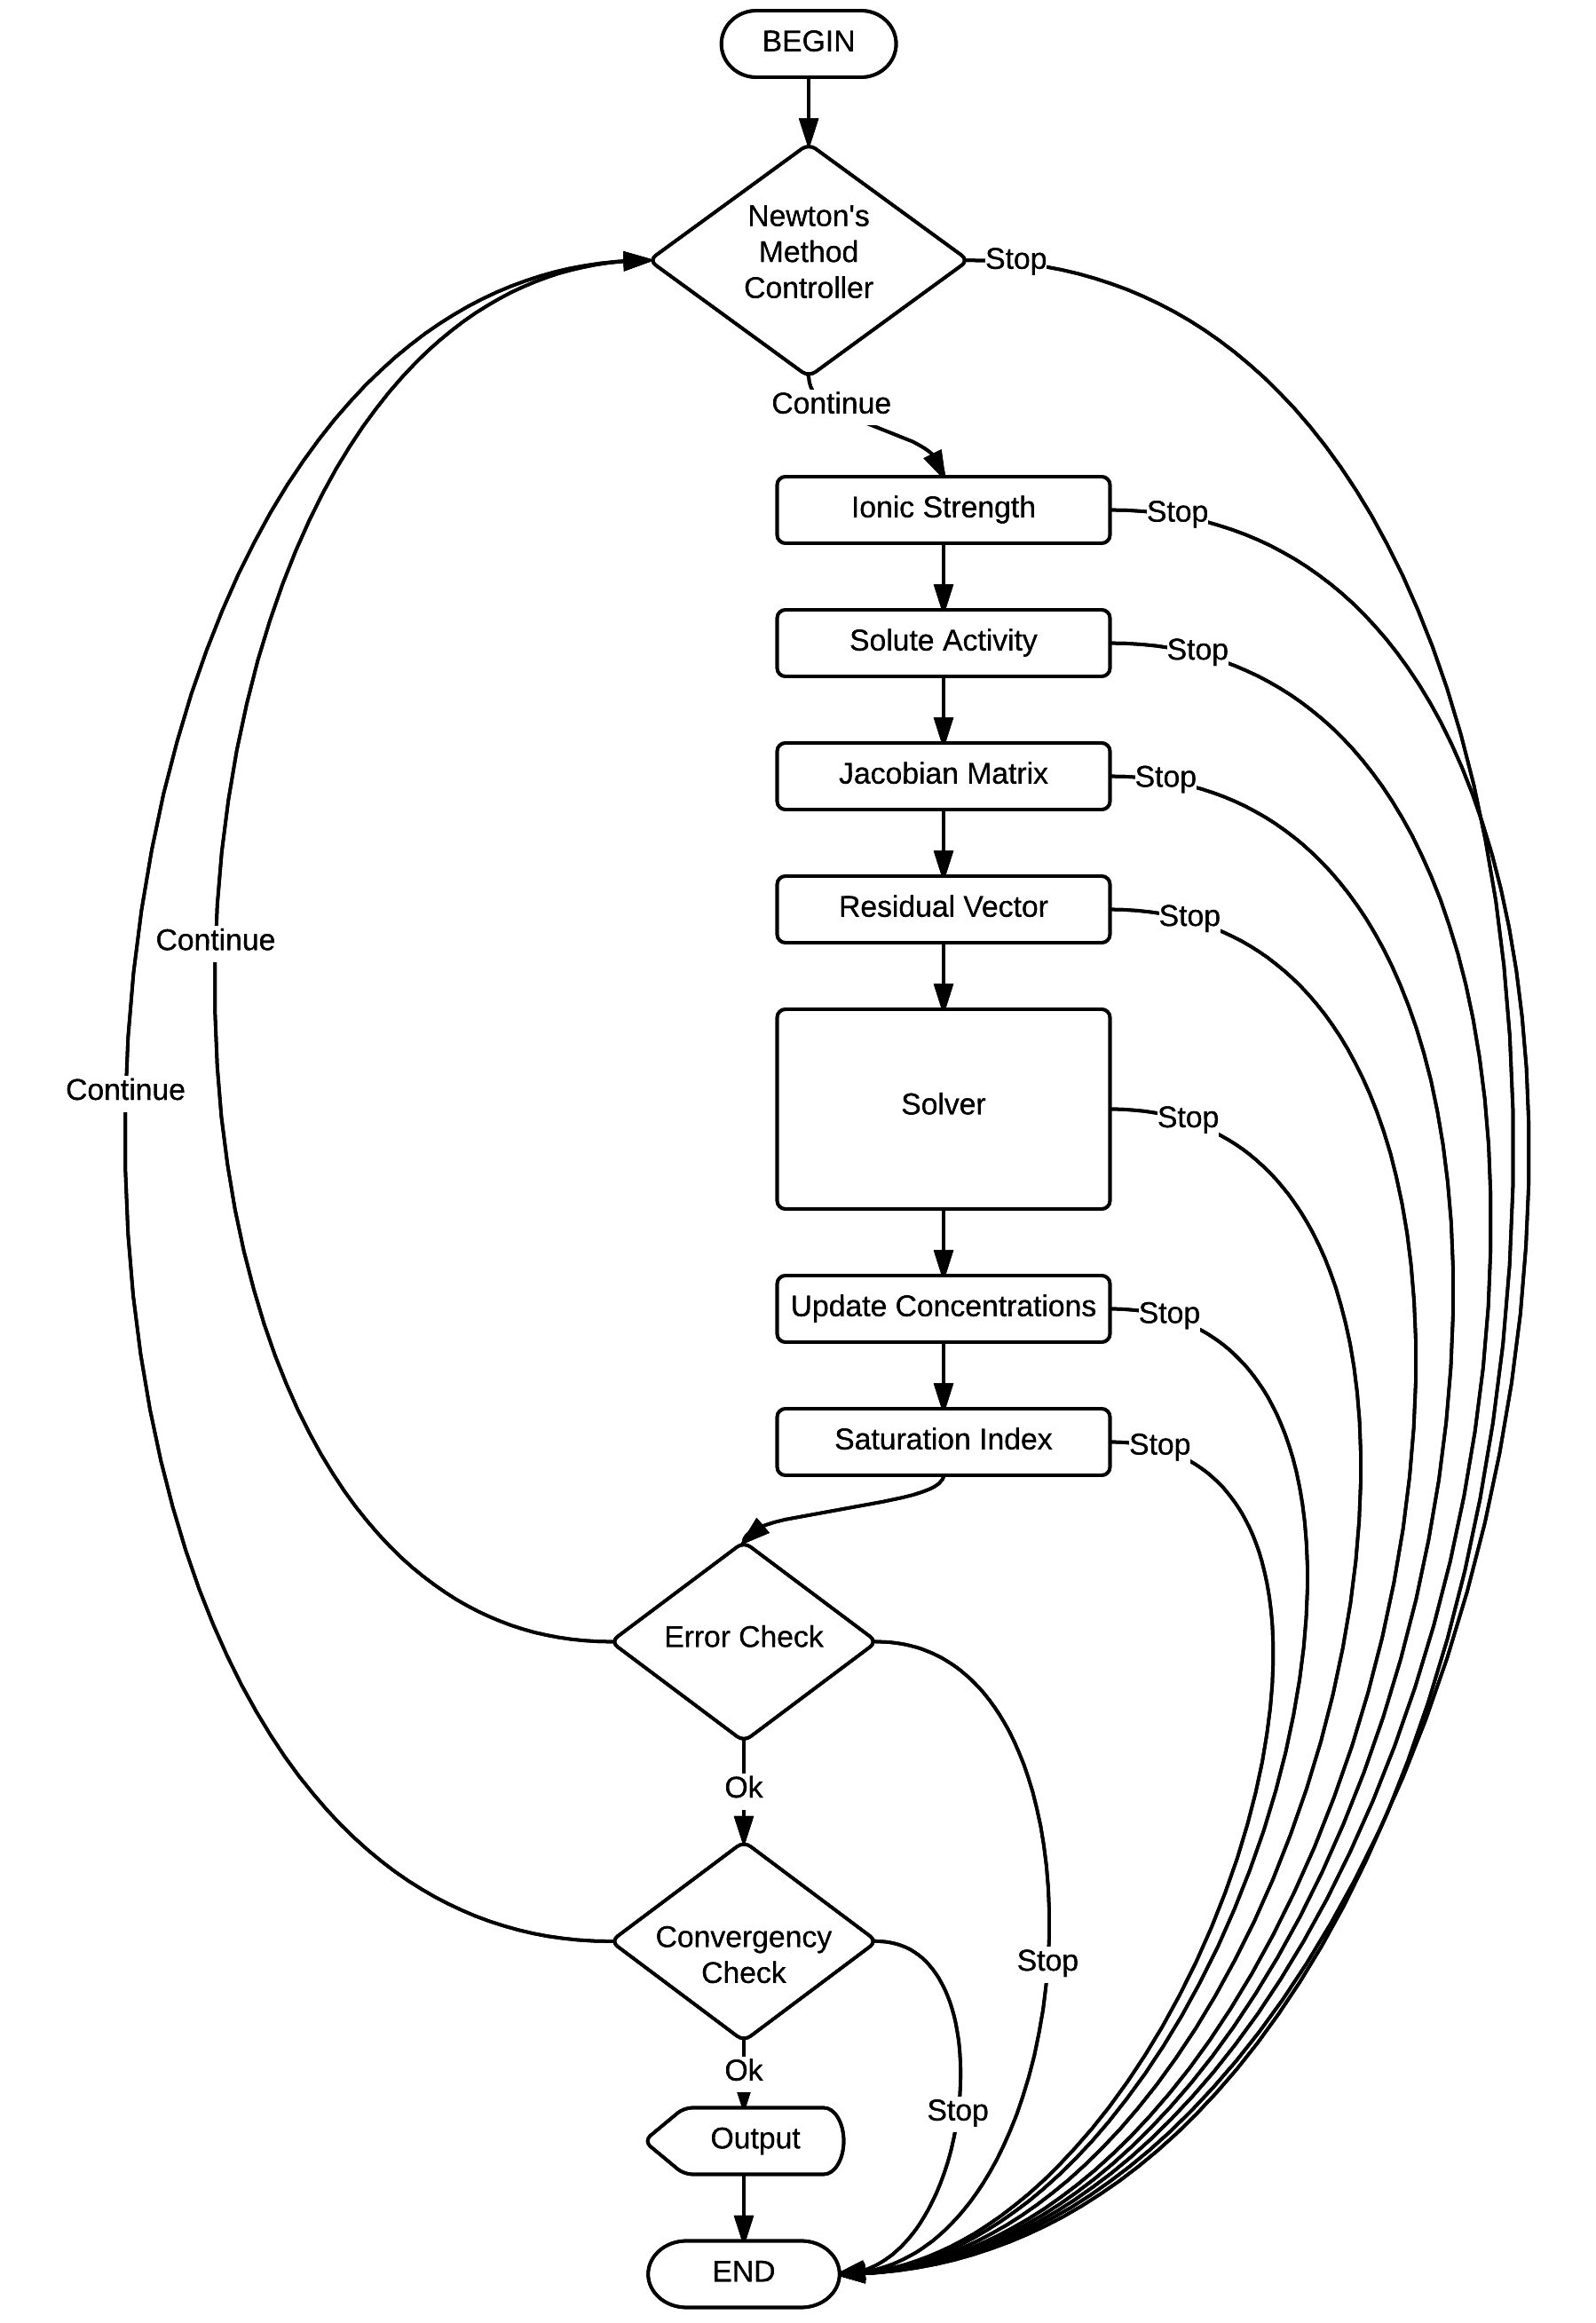
\includegraphics[width=100mm]{figures/Shpeck_algo_newton.png}
\caption{Algorithm of the Newton's Method Solver}
\label{fig:Shpeck-algo-newton}
\end{figure}
\subsection{Complexity of the algorithm}
The Gauss-Newton's method has a complexity O($n^3$) per iteration with a quadratic convergence.

%(http://ranger.uta.edu/~huber/cse4345/Notes/Nonlinear_Equations.pdf)
%(http://ranger.uta.edu/~huber/cse4345/Notes/Equations.pdf)
%(compared to http://en.citizendium.org/wiki/Newton%27s_method#Computational_complexity)


\section{Graphical User Interface}
Due to the enormous amount of options connected to the nature of geochemical modeling, the development of a GUI is a challenge itself. It is necessary to develop a software that is intuitive and user-friendly and has an accurate and efficient approach to all of the options available in nature and the system. The development of the GUI introduces several stages of processes related to it:
\begin{itemize}
	\item Planning : This moment is where the developer needs to think a way to contemplate all the options from the core of the program and make them easily, intuitive and friendly to the final user. The planning is an essential process and must be correct. All the content, features, details of the software need to be strictly defined and organized in order not to break anything afterwards nor forget it (which will result in a not used software). A slight path divides something really useful from something not useful at all - assumptions and the challenge of the developer to think as a user is sometimes tough because many of the developers are not the final user for its applications. Is important also to find out what others have done or are doing - during the study of others software their GUI were analyzed carefully.
	\item Building : All the planning done for needs to be implemented and the main features of the software are important to be well defined at this point. To build the tool \emph{Qt} - already presented above - was chosen due to its many advantages as easy to customize; no coding; templates; simple drag and drop \emph{GUI}  builder; secure and reliable;
	\item Ensuring Usability : The challenge in the field of Human-Computer Interaction (HCI) investigates way people use computers is huge. Techniques and tools are used to find some relevant standards, and some measurements are available. Just to name a few, tests with real users; evaluation by experts; gathering user feedback; Usage logging;
\end{itemize}


\subsection{\emph{SHPECK}'s GUI }
Among geochemical modelling software, the GUI was either not or poorly implemented. We see\emph{SHPECK} as geochemical speciation modelling software with a potential to broaden its influence. The \emph{GUI} enables the user to focus on essential duties and not struggle with the mental power wasted on things that do not matter when modelling a geochemical environment. We think of the GUI with a bright idea that the less skill it requires, the better it is.
\emph{SHPECK}'s GUI works based on tabs, each tab is responsible for viewing an specific point of the software. We present them in details bellow:
\begin{itemize}
\item Configurations tab: Allows users to view and manipulate basic system settings and controls such as temperature, activity coefficient calculation method, the number of iterations, solver options, maximal error and convergence criteria. It is presented in ~\ref{fig:config}.
\item Compounds in the water tab: Allows users to create and edit the composition of the water that will be used in the geochemical speciation model. It has  all the species available from the database and its concentration. The species in the tab that have concentration different than zero compose the water. This tab is presented in ~\ref{fig:water}.
\item Results tab: Allows the user to see relevant input information and the outputs of the geochemical speciation model such temperature, ionic strength, pH of the solution, final concentration for the species, saturation indexes, etc. It is presented in ~\ref{fig:output}
\end{itemize}


\begin{figure}[ht!]
\centering
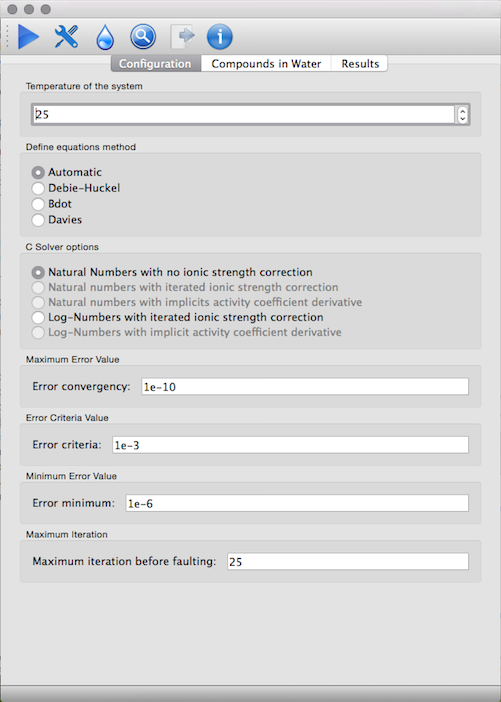
\includegraphics[width=100mm]{figures/shpeck-configtab.png}
\caption{Configuration tab}
\label{fig:config}
\end{figure}

\begin{figure}[ht!]
\centering
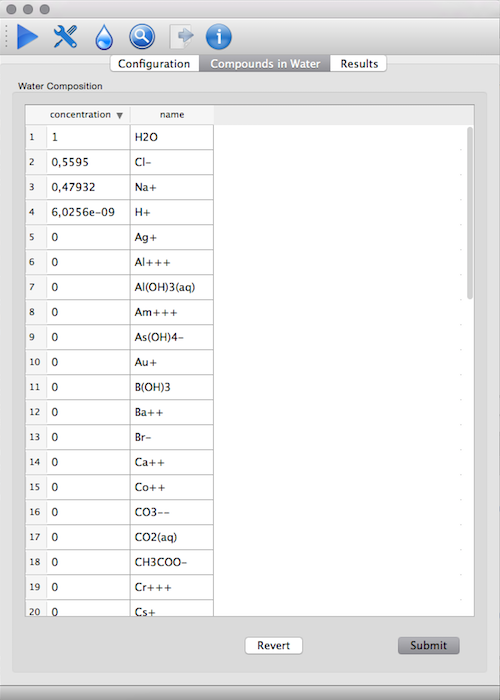
\includegraphics[width=100mm]{figures/shpeck-watertab.png}
\caption{Water composition tab}
\label{fig:water}
\end{figure}

\begin{figure}[ht!]
\centering
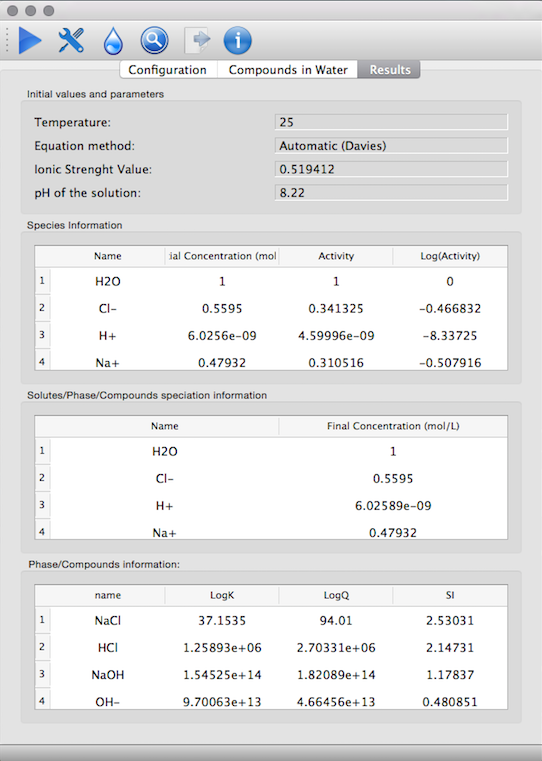
\includegraphics[width=100mm]{figures/shpeck-resultstab.png}
\caption{Results tab}
\label{fig:output}
\end{figure}

\section{Database}
As can be seen in this chapter, the algorithm of \emph{SHPECK} is not trivial and requires many interactions between many different entities. The database is responsible for providing all the data that will flow through and works as the \emph{seed} provider. Chapter ~\ref{chapter:review} makes clear that using a flat file database is something harmful to the software. Potential issues of using flat file databases are duplication of the information; non-unique records; hard to update; inherently inefficient; harder to change data format; poor at complex queries; no security;
In \emph{SHPECK}, we use a relational database, which is a model of a database that prevents all the problems faced in flat file database previously discussed and enable to take full advantage of the information on it. Relational databases work based on a \emph{query}, which is an information request from the database. Besides that, there are three important advantages:
\begin{itemize}
\item A relational database has the advantage of not necessarily be in the memory of the computer - often these databases are larger than the computer's memory. What happens is that the software fetches the information on-the-go. 
\item Complex queries enable the versatility and efficiency when fetching relevant information from the database. Instead of scanning the whole flat file, the query can pre-define the categories of information - even from multiple tables - which will be sought. Also important to mention, a query can be composed and concatenated on runtime execution - meaning that \emph{SHPECK} only fetches from the database information relevant to the specific simulation that is being executed (species, compounds, reactions, etc.). Complex queries and concatenation of queries result in a faster and more efficient use of the available resources.
\end{itemize}

Instead of being something to worry about, the database is one of the most critical and significant infrastructure parts of our software. The database architecture was defined after studying the algorithm and determining what would be the structure and the information needed - it is presented in details in figure ~\ref{fig:ERDiagram}. We developed a relational database that embrace all the important data already in use from other software but with a newer approach and structured in tables - naturally some changes in the structure were necessary in order to compact, organize, structure and make it easier to use.

\begin{figure}[ht!]
\centering
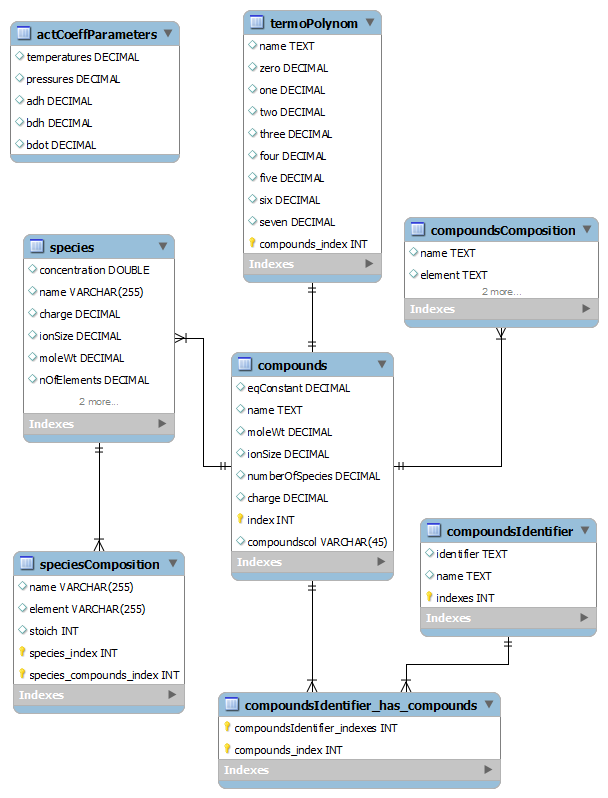
\includegraphics[width=100mm]{figures/ER_diagram.png}
\caption{ER Diagram of the database}
\label{fig:ERDiagram}
\end{figure}

\subsection{Database Technologies}
We use the SQLite database \cite{SQLite}, which is a software library that implements a self-contained, transactional \emph{SQL} database engine, open source and currently is the most widely deployed \emph{SQL} database engine in the world. Some of its advantages are explained bellow:
\begin{itemize}
\item Zero-Configuration: \emph{SQLite} does not need to be installed before it is used, there is no setup procedure;
\item Serverless: The process that wants to acess the database reads and writes directly from the database files on disk. There is no intermediary server process (nor interprocess communication using \emph{TCP/IP});
\item Single Database File: An \emph{SQLite} database is a single file located in the directory hierarchy. \emph{SQLite} database can be easily copied onto a USB memory stick or emailed for sharing;
\item Stable Cross-Platform Database File: A database file written on one machine can be copied and used on a different machine with a different architecture. Furthermore, \emph{SQLite} is backwards compatible (newer versions can read and write older database files);
\end{itemize}

\subsection{\emph{LLNL} thermodynamic dataset parser}
Once we defined what would be the structure and the technology of our database, we need to find the information to populate it - the information that would  feed \emph{SHPECK}. We create a parser for the flat file database that extracted the information and arranged it following our structure. 
The parser was carefully generated in order not to misunderstand any structure nor miss a delimiter - this task was extremely time-consuming and proportionally important for the success of \emph{SHPECK}.

\newpage


\section{Summary}
\begin{itemize}
\item Architecture: \emph{SHPECK} follows the architectural pattern called \emph{MVC}; It's benefits are the complete separation of responsibilities and concerns among the parts of the software; there is no mixing of codes between them. Another advantage that worth mentioning is the flexibility for the software to grow and develop itself. Figure ~\ref{fig:shpeck-architecture} displays the \emph{MVC} pattern existing in \emph{SHPECK}.
\item Governing Equations: \emph{SHPECK} is a geochemical speciation modelling software that drives the behaviour of the aqueous system based on a set of mass-action equations combined with equilibrium constraints. A mass-action equation is described in equation  ~\ref{eq:massaction} and reinforced here:

\begin{equation}
K_j =  \prod\limits_{i=1}^N  a_i^{v_{ij}} \hspace{35pt}    (j = 1, ... , M)
\end{equation}

where $K_j$ denotes the equilibrium constant of the \emph{j-th} reaction; $a$ denotes the activity of the \emph{i-th} chemical species.

\item Numerical Method: \emph{SHPECK} applies the \emph{Gauss-Newton's} method to solve the nonlinear system of equations. The concept of the method is described in equation ~\ref{eq:gaussNewtonMethodEq1} and reinforced here:

\begin{equation}
F(x+1) = F(x) - J^{-1} * R
\end{equation}

Where $F$ is function's result for the applied $x$, $J^{-1}$ is the inverse of the Jacobian matrix, and $R$ is the residual matrix. The quadratic rate of convergence of this method compensate the expensive calculation inherent to it.

\item Graphical User Interface: The \emph{GUI} mission is to enable the user to use fully the potential \emph{SHPECK} has to offer. It is intuitive and user-friendly to allow the user to focus on essential duties that are imperative to model a geochemical environment. We use the popular approach of \emph{tab} panels, which are separated according the purpose of it: configurations and settings, water composition and results visualization.
\item Database: A geochemical modelling software is severely dependent on the information inside it. \emph{SHPECK} structure all of its data in a \emph{SQLite} relational database, unique among the commercial software available. \emph{SHPECK}'s database is composed by the information about elements, species, compounds, reactions and thermodynamic constants from the \emph{LLNL} thermodynamic dataset. A parser for \emph{LLNL} flat file database was created to fetch this information.
\end{itemize}
\newpage
%%%%%%%%%%%%%%%%%%%%%%%%
%                                                                       %
% Verification and Validation   %
%                                                                        %
%%%%%%%%%%%%%%%%%%%%%%%%%

\chapter{Verification and Evaluation}
\label{chapter:validation}
%COMMENTED OUT AFTER TONY's REVIEW
%TONY: In this section, all you are doing is testing if your program generates a similar results as given by another program. There is no need to talk about the geological model or problem. Talking about diagenesis and any implication to petroleum system is out of question.

%During the development of this work, we have always been in contact with geochemists to present them the partial results of our geochemical speciation modeling software. We collected feedbacks regarding how to achieve a better software, as well as checking if our solution is fulfilling its purpose with consistent results. \\
%As final evaluation of this work, we selected an application relevant to petroleum systems. Many physical-chemical reactions happens during the generation, migration and storage of oil. \emph{Diagenesis} is the definition of the several processes that are involved and it is driven by multiple factors as temperature, pressure, mineral composition, water composition, activity of the solutes, pH, etc. 
%The \emph{diagenesis} is responsible for compaction and precipitation of minerals \cite{Tucker:01} and therefore, porosity, solubility and permeability of these reservoirs. The study of diagenesis is important because it allows to understand the geologic history of rocks, specially sedimentary rocks. In sedimentary rocks, the deposition of sediments are compacted in different layers and cemented by minerals that precipitate from reactions in a chemically very active environment. The \emph{diagenesis} reactions happens because the components are always trying to reach equilibrium, and therefore, they tend to interact with each others \cite{Burley:85}.
%Using geochemical modeling softwares is a powerful tool to understand the diagenetic processes and the natural conditions that occur in this natural environment. The goal is to numerically model this environment and analyse the results of the diagenetic reactions with a petrographic analysis of the modeled reservoirs.


%Análise geologica da aplicação do SHPECK feita pela Mara

In order to test and evaluate the simulator, we model the diagenetic reactions observed in Snorre Field reservoir sandstones of Norwegian North Sea. The main reservoir horizons of the field are the fluvial sandstones in the upper member of the Upper Triassic Lunde Formation and the Upper Triassic to Lower Jurassic Statfjord Formation \cite{Hollander:87}. The sandstones sampled for this study, according to Morad \cite{Morad:90}, belong to the upper member of the Lunde Formation. The sandstones are dominantly fine to  medium-grained and arkosic, with framework constituents of quartz (40-80\%), K-feldspar (5-12\%), plagioclase (15-45\%), muscovite, biotite and clay minerals that include smectite, mixed-layer clay minerals, chlorite and subordinate amounts of kaolinite and illite. Subordinate rock fragments include intraformational mudstone and carbonate clasts and extrabasinal grains of quartz-feldspar-mica aggregates that probably represent granitic rocks and/or schist or gneisses. Mica and detrittal clay minerals seldom make up more than 2\% of the total mineral content in the sandstones. Diagenetic clay minerals include pore-filling kaolinite and pore-lining smectite, mixed-layer chlofite-smectite, and chlorite. Other cements include the carbonates (0.0-25\%) which play a significant role in porosity reduction in some of the sandstones. Authigenic overgrowths are primarily quartz, anatase and minor albite, pyrite and barite.

\section{Case Study}
For the model’s validation, the diagenetic reactions observed in Snorre Field reservoir sandstones, Norwegian North Sea were simulated. Morad~\cite{Morad:90} modelled the diagenetic reactions that take place in the Snorre Field. The modeling set up and results given by this author describe the texture, origin, chemistry of the sandstones reservoirs in terms of the water composition and temperature.The description of the diagenetic reactions and these data allowed us to generate a computationally comparative study and, consequently, to validate \emph{SHPECK}'s results. 


We model and compare the same diagenetic environment using \emph{SHPECK}, \emph{PHREEQC} and \emph{MINTEQA2}. The water composition is detailed in \cite{Nordstrom:79}.


We approach the environment described above following two methodologies: experimental and computational. The first one analyzes and compare the behavior of \emph{SHPECK} with petrographic analysis through thin sections (available in \cite{Morad:90}). The second treats the direct comparison of \emph{SHPECK}'s results side-by-side with other software's.

\subsection{Experimental validation of Shpeck}
As stated in \cite{Morad:90}, the model presented in \cite{Egeberg:88} calculates activities of the various ions of formation waters using the ion association model (originally described in \cite{Wigley:77}). The thermodynamics data used in this modeling are given in \cite{Helgeson:74a},  \cite{Helgeson:74b}, \cite{Helgeson:76}, \cite{Waltter:77}, \cite{Helgeson:78} and \cite{Helgeson:81}.


The activity diagram generated for a known temperature and log activity ratio of Potassium to Sodium ions of \cite{Aagaard:90}  is provided as input to \emph{SHPECK} (Figure ~\ref{fig:tempXactratio}). The results show a consistent pattern: as the temperature rises the potassium activity gets higher over sodium’s, which means that the phases associated to the ion potassium (i.e. K-feldspar, Illite, etc) are dissolving.


\begin{figure}[ht!]
\centering
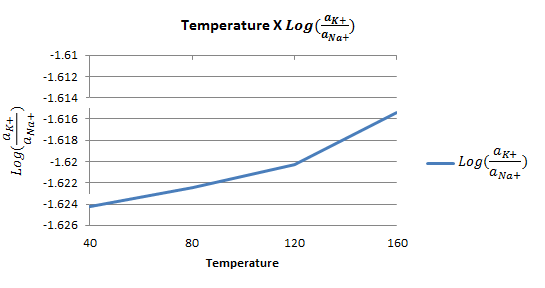
\includegraphics[width=100mm]{figures/tempXactratio.png}
\caption{Log activity ratio of Potassium to Sodium ions using the results from \emph{SHPECK}}
\label{fig:tempXactratio}
\end{figure}



\subsection{Computational comparative study} 
By modeling the same environment using three distinct software packages, we attain a relevant comparison among the numerical methods and algorithms. 


The chemical composition of the water adopted in the models is taken from  \cite{Nordstrom:79}, which provides the chemical composition of the seawater (Table ~\ref{tab:nordstrom}). The comparative study tested temperatures that have varied from $100^o$C to $100^o$C. In \emph{MINTEQA2}, due to limitations of its thermodynamics equilibrium database, the maximum temperature available is $100^o$C.

\begin{table}
\caption{Chemical composition of the solution in the seawater at $25^o$ in $mM/L$C }
\label{tab:nordstrom}
\centering
\begin{tabular}{r|c|c|c|c|c|c|c|c|c}
\ce{Al^{3+}} & \ce{K^+} & \ce{Na^+} & \ce{Ca^{2+}} & \ce{Mg^{2+}} & \ce{Fe^{2+}} & \ce{SiO_2}&  
\ce{SO_4^{2-}} & \ce{Cl^-} & pH
    \\ \hline
7.59e-5 & 10.45 & 479.32 & 10.53 & 54.39 & 3.66e-5 & 0.073 & 28.893 & 559.5 & 8.22
\end{tabular}
\end{table}

We aim to model the diagenetic processes that best represent the behavior of ions in the water-rock interactions. Figures ~\ref{fig:na+},~\ref{fig:cl-},~\ref{fig:mg+2} and ~\ref{fig:ca+2} present the most representative ions of the solution. 


It is possible to see that the behavior of \emph{SHPECK} is similar to  both \emph{PHREEQC} and \emph{MINTEQA2} in most of the cases, especially in temperatures under $100^o$C. We observe a more dissimilar behavior between \emph{SHPECK} and \emph{PHREEQC} in temperatures higher than $100^o$C, but the results were never completely opposite. This can be explained by the temperature intervals where the equilibrium constant \emph{K} is not completely defined. This is a known issue from the \emph{LLNL} thermodynamic dataset: sometimes equilibrium constants have no measures in literature and are treated as unknown. \emph{SHPECK} adopts the nearest equilibrium constant known value. Unfortunately we do not have access to the whole software’s details in order to describe how they treat this issue.

\begin{figure}[ht!]
\centering
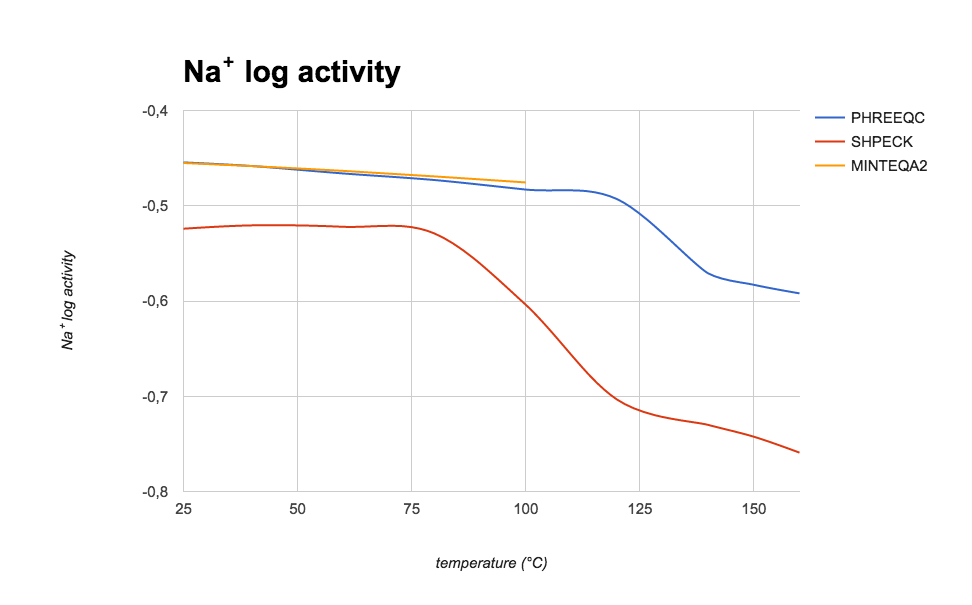
\includegraphics[width=140mm]{figures/na+.png}
\caption{\ce{Na^+} log activity comparative study}
\label{fig:na+}
\end{figure}

\begin{figure}[ht!]
\centering
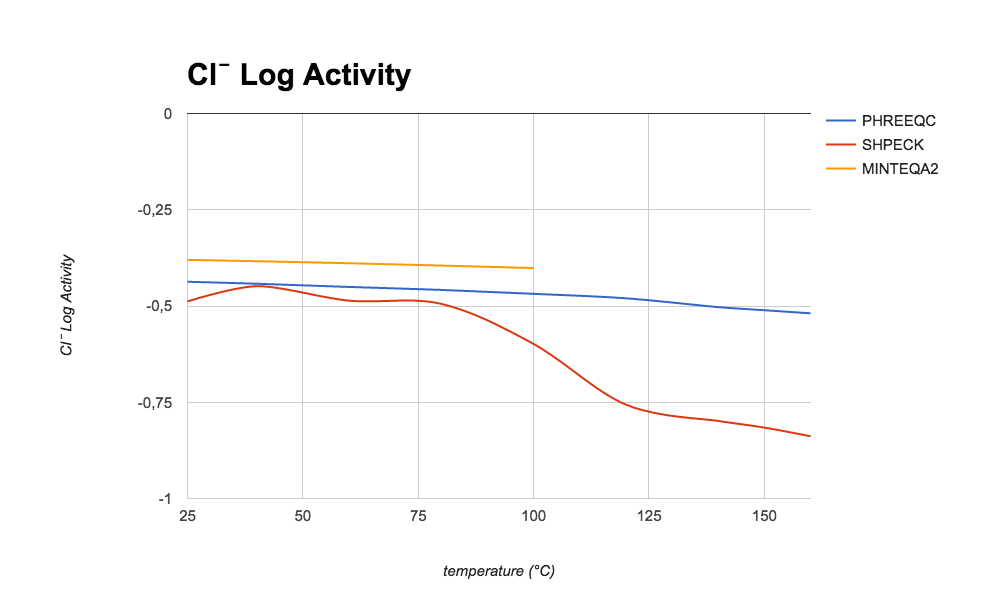
\includegraphics[width=140mm]{figures/cl-.png}
\caption{\ce{Cl^-} log activity comparative study}
\label{fig:cl-}
\end{figure}

\begin{figure}[ht!]
\centering
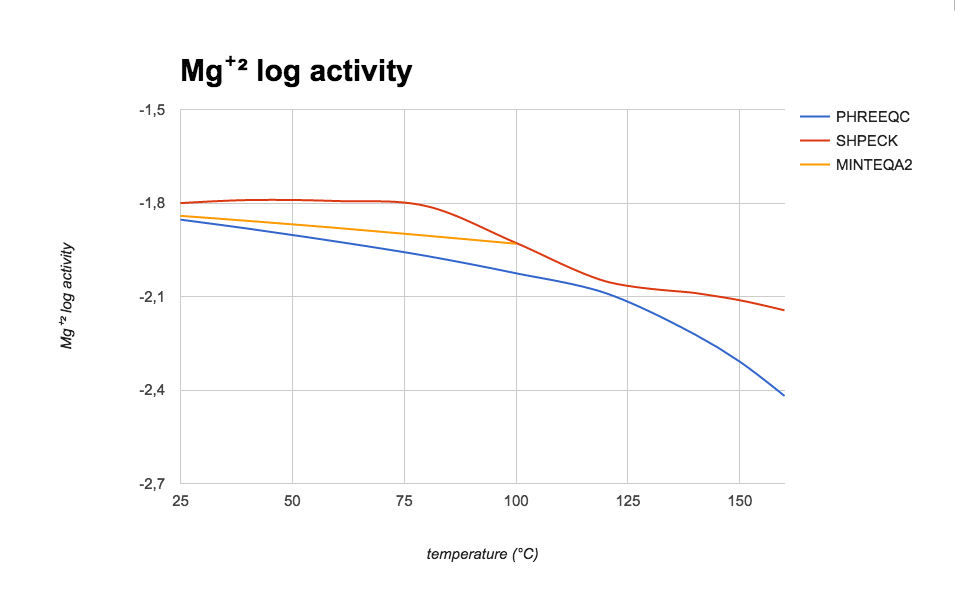
\includegraphics[width=140mm]{figures/mg+2.png}
\caption{\ce{Mg^{+2}} log activity comparative study}
\label{fig:mg+2}
\end{figure}

\begin{figure}[ht!]
\centering
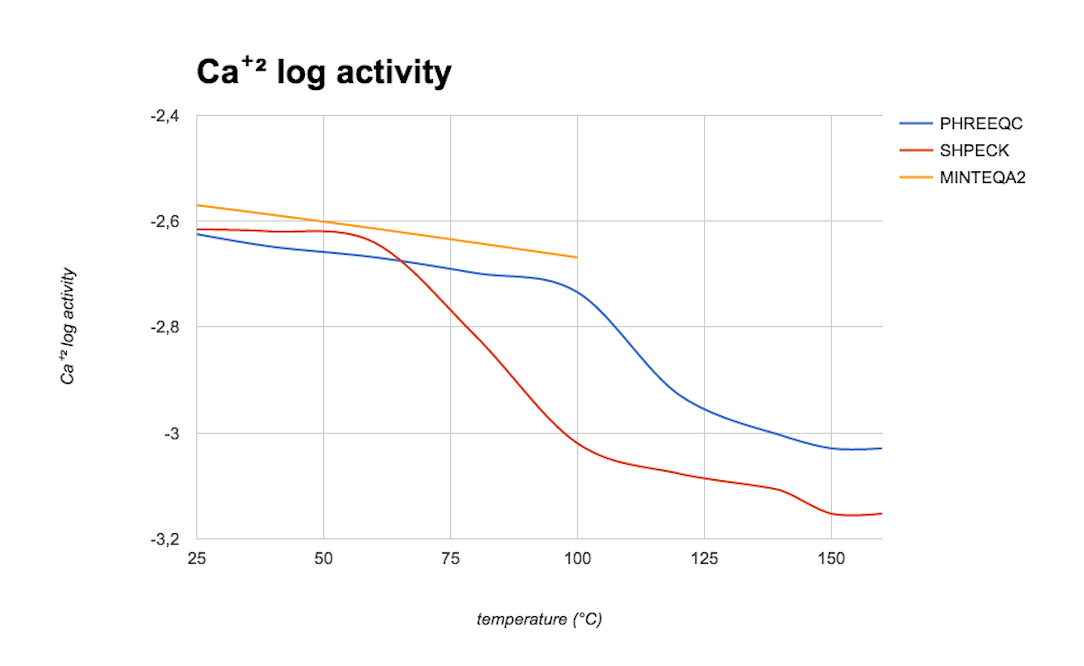
\includegraphics[width=140mm]{figures/ca+2.png}
\caption{\ce{Ca^{+2}} log activity comparative study}
\label{fig:ca+2}
\end{figure}

\begin{figure}[ht!]
\centering
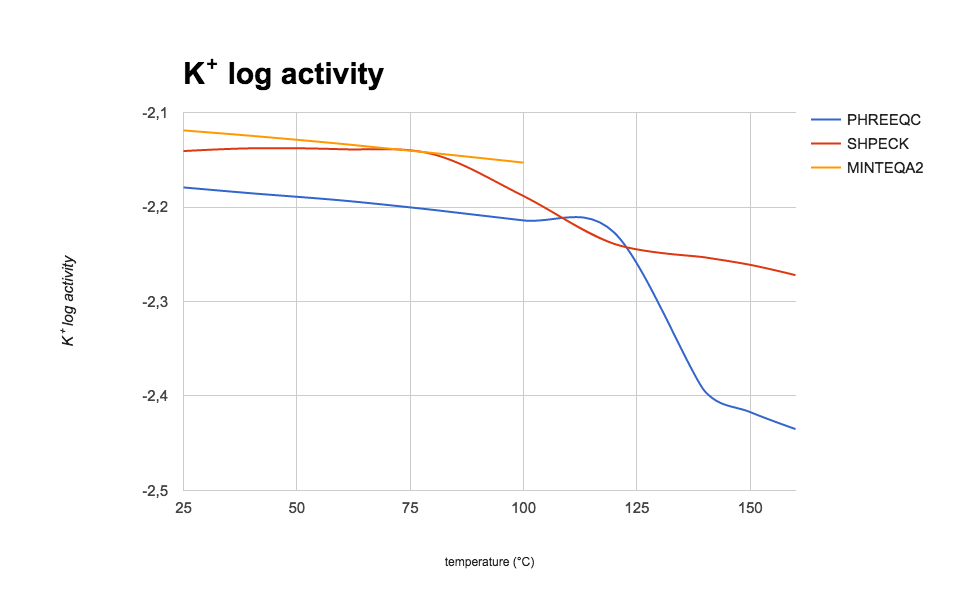
\includegraphics[width=140mm]{figures/k+.png}
\caption{\ce{K^+} log activity comparative study}
\label{fig:k+}
\end{figure}

\begin{figure}[ht!]
\centering
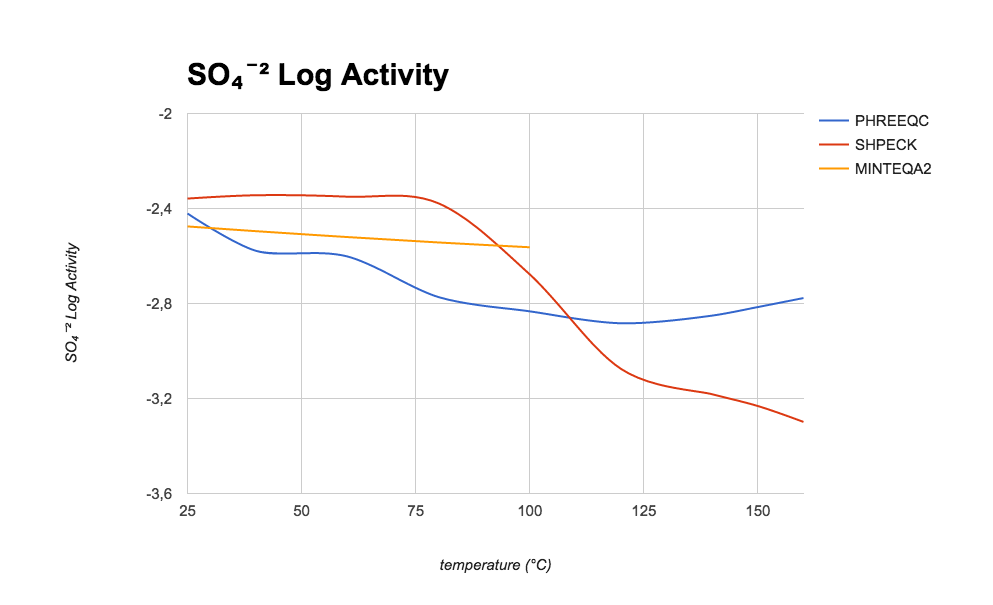
\includegraphics[width=140mm]{figures/so4-2.png}
\caption{\ce{SO_4^{-2}} log activity comparative study}
\label{fig:so4-2}
\end{figure}


\section{Database Evaluation}
The geochemical modeling tools used in our comparison studies use text files as databases. 
The goal of this section is to make clear the difference and - more importantly - the benefits of \emph{SHPECK}'s relational database. 
Most of the information inside a geochemical database is related to each other (i.e. a mineral phase is described by a reaction, a reaction is composed by solute species, and a solute species is composed of chemical elements).


\emph{SQLite} databases are naturally a structure where the data can be related to each other, and this significantly improvements the performance and robustness of the application. On \emph{SQLite} databases, the data can be accessed using \emph{SQL} queries that reduce the complexity and increase the speed on information retrieval. Code~\ref{cod:sqlQuery} shows a typical query issued from \emph{SHPECK}'s \emph{SQLite} query. Text database files only allow sequential access to the information that it contains. In relational databases, the \emph{SQL} language allows to selectively locate the needed data.


\begin{minipage}{0.8\linewidth}
\begin{lstlisting}[frame=single, label=cod:sqlQuery, caption=\emph{SHPECK}'s \emph{SQLite} example query. The value ”XXXX” is updated to the simulation’s solute name.]
SELECT compoundsComposition.element, compoundsComposition.name, compoundsComposition.stoich, compounds.eqConstant, termoPolynom.zero, termoPolynom.one, termoPolynom.two, termoPolynom.three, termoPolynom.four, termoPolynom.five, termoPolynom.six, termoPolynom.seven FROM termoPolynom, compoundsComposition, compounds WHERE compoundsComposition.name = compounds.name AND termoPolynom.name = compounds.name AND compounds.name = XXXXX;
\end{lstlisting}
\end{minipage}

It is interesting to point out that with Code~\ref{cod:sqlQuery} the information is fetched from three different tables; so, with only one query, many relevant information for the simulation is retrieved.

\subsection{Configuration setup}
For evaluating the time advantage of using a database in SPHECK, we have taken time measures of how long the program was idle waiting for this information and when it finally was available. In both the relational database and flat file experiments, we used the \emph{NNLN} thermodynamic dataset. 


At first, we defined what was the information necessary from the database to generate the set of reactions. After that, we established the order in which this information was needed and how to fetch it.  


The tests were executed on a MacBook air, i7 processor, 1.7GHz, 8GB RAM running OS X 10.9.3.

\subsection{Time analysis of fetching information}
The objective of the time analysis is to measure how long it takes to fecth the same information from different types of database. The response time is considered as the sum of the processing time and the time waiting for the availability of the resource. It is necessary to understand that until the software has received the information requested from the database it is inactive and in a standby mode. In order to analyze the response time within a geochemical analysis point of view, we discuss not only the access time but also the implications of that information. 


When fetching any information from a thermodynamic dataset, it is important to take into consideration additional data will also have to be retrieved. For example, when fetching a reaction (as expressed in Equation~\ref{reaction}) data, the basic information consists of the compounds that take part on this reaction and the related stoichiometric values. Behind this action, the database must also provide information about the compounds itself (i.e. charge, ion size, mole weight, elements in that specie, formula, mole volume) as well as the reaction (i.e., thermodynamic equilibrium constant coefficients, etc).

Figure ~\ref{fig:timeXaccess} indicates the time elapsed (in seconds) that it takes to retrieve the necessary information related to a chemical reaction from the database. In this example, we simulated from 20 to 580 randomly selected reactions in the database. It is possible to observe that \emph{SHPECK}'s database has improved approximately 40\% in the average time elapsed to fetch the information if compared to the regular text file databases used by other simulation packages.

\begin{figure}[ht!]
\centering
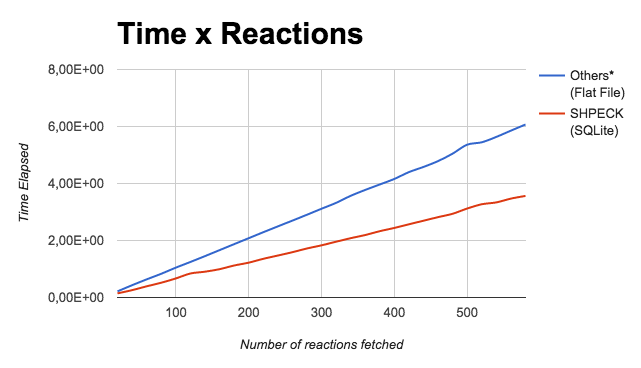
\includegraphics[width=140mm]{figures/timeXreactionAccess.png}
\caption{Time elapsed in seconds X Reactions Accessed}
\label{fig:timeXaccess}
\end{figure}

\newpage

\section{Summary}
\begin{itemize}
    \item Diagenesis: This term refers to chemical and physical changes taking place in a rock due to chemical reactions. In this study we reproduce the diagenetic reactions observed in Snorre Field reservoir sandstones, Norwegian North Sea. 
    The environment modeled is described in \cite{Morad:90} and the chemical composition of the water in \cite{Nordstrom:79}.
    \item Comparative study: We performed a comparative study of \emph{SHPECK} and other available geochemical speciation software. The results prove that \emph{SHPECK} produces comparable results. The discrepancies are minimal and the differences can be justified by the software-specific implementations of the mathematical and computational treatment to the set of equations and other parameters. 
    \item Database evaluation: The lack of a relational database in other geochemical modeling software makes it clear that none of the existing options were developed with emphasis on a computer science emphasis. \emph{SHPECK} uses a \emph{SQLite} database specially developed to support a geochemical speciation modeling software. This design option enables the software to achieve efficient performance, and handle complex data queries and retrieval. A comparative plot highlights the advantages in elapsed time by the number of reactions requested.
\end{itemize}
\newpage
%%%%%%%%%%%
%                            %
% CONCLUSION   %
%                            %
%%%%%%%%%%%

\chapter{Conclusion}

Geochemical speciation is critical for understanding the form of chemicals of interest in natural systems. It is crucial in many different aspects of our daily life nowadays: assessing bioavailability, risk to humans and ecosystems. Geochemical speciation models are generaly determined through analytical methods that measure free ions or total concentrations, used in conjunction with thermodynamically based models. As presented on this work, these models rely on the local equilibrium assumption, and on experimentally determined reaction constants. It is clear, though, that if the chemical system does not achieve equilibrium state or if the equilibrium constants are not certain, the geochemical speciation model's prediction show significant uncertainty.
This emphasizes the clear need for a proper computation approach while treating with such influential information like a geochemical speciation model. The information flow is tightly connected and any mistake will propagate errors and carry that wrong information until the very end of the model.

As computer simulation methods have gained importance in more and more disciplines, the issue of their trustworthiness for generating new knowledge has grown; therefore, we present an interesting study case where is possible to absorb and realize the comprehensiveness of this work.

Calculation of speciation is conducted by substitution of the equilibrium constants into the mass balance expressions for the total concentration of a particular component. This results in a series of nonlinear equations which are solved iteratively using numerical techniques, such as the Newton-Raphson iteration used in the MINTEQA2 model. Iterations continue until the total calculated component concentrations, derived from the equilibrium expressions, calculated activity coefficients, and component mass balances, and the measured total concentrations converge to a prescribed limit.

\begin{itemize}
\item Review of the results emphasizing our approach and advantages
\item  Geological explanations for the results
\item  Final discussion about \emph{SHPECK}
\item  CONTRIBUTION (EXPLICIT AND WELL DESCRIBED) 
\end{itemize}


%This work provides three important steps of the development of a geochemical modeling speciation software with the purpose of increasing the quality in such field of softwares. The development of a new software is intended to raise and optimize in every possible way the concept of geochemical modelling always taking into account the computer science priorities and theory. The difference between all the options and this work's approach is that the computer science's side is taken more responsibly and strategically thought since the beginning. What have been notested from all existing softwares studied is that they were created by geochemists, chemicals, geologists to solve their daily challenge and questions - our approach is different: it is done by computer science specialists with the support of geologists and geochemicals. Naturally some challenges are faced, for example, the base concepts are sometimes misunderstood and it is mandatory that the basic concepts are well stablished in order to have a solid and useful software in the end of the process. During the process of developing this work aspects of physical chemistry, aqueous geochemistry, linear algebra, complex coupled systems and computational simulatosrs are going to be studied and learned.
\newpage

% references
\bibliography{references}
\bibliographystyle{inputs/abnt-ufrgs}      % Procura pelo arquivo "abnt-ufrgs" - normas ABNT.
\clearpage

\appendix
/** Disk-Space Utilization Report For shpeck_database_august

Page size in bytes................................ 1024      
Pages in the whole file (measured)................ 399       
Pages in the whole file (calculated).............. 277       
Pages that store data............................. 258         64.7% 
Pages on the freelist (per header)................ 19           4.8% 
Pages on the freelist (calculated)................ 141         35.3% 
Pages of auto-vacuum overhead..................... 0            0.0% 
Number of tables in the database.................. 9         
Number of indices................................. 0         
Number of defined indices......................... 0         
Number of implied indices......................... 0         
Size of the file in bytes......................... 408576    
Bytes of user payload stored...................... 196622      48.1% 

*** Page counts for all tables with their indices *****************************

TERMOPOLYNOM...................................... 93          23.3% 
COMPOUNDSCOMPOSITION.............................. 85          21.3% 
COMPOUNDS......................................... 44          11.0% 
COMPOUNDSIDENTIFIER............................... 23           5.8% 
ELEMENTS.......................................... 3            0.75% 
SPECIES........................................... 3            0.75% 
SPECIESCOMPOSITION................................ 3            0.75% 
SQLITE_MASTER..................................... 3            0.75% 
ACTCOEFFPARAMETERS................................ 1            0.25% 

*** Page counts for all tables and indices separately *************************

TERMOPOLYNOM...................................... 93          23.3% 
COMPOUNDSCOMPOSITION.............................. 85          21.3% 
COMPOUNDS......................................... 44          11.0% 
COMPOUNDSIDENTIFIER............................... 23           5.8% 
ELEMENTS.......................................... 3            0.75% 
SPECIES........................................... 3            0.75% 
SPECIESCOMPOSITION................................ 3            0.75% 
SQLITE_MASTER..................................... 3            0.75% 
ACTCOEFFPARAMETERS................................ 1            0.25% 

*** All tables ****************************************************************

Percentage of total database......................  64.7%    
Number of entries................................. 6403      
Bytes of storage consumed......................... 264192    
Bytes of payload.................................. 197816      74.9% 
Average payload per entry......................... 30.89     
Average unused bytes per entry.................... 4.81      
Average fanout.................................... 31.00     
Maximum payload per entry......................... 185       
Entries that use overflow......................... 0            0.0% 
Index pages used.................................. 8         
Primary pages used................................ 250       
Overflow pages used............................... 0         
Total pages used.................................. 258       
Unused bytes on index pages....................... 6088        74.3% 
Unused bytes on primary pages..................... 24735        9.7% 
Unused bytes on overflow pages.................... 0         
Unused bytes on all pages......................... 30823       11.7% 

*** Table ACTCOEFFPARAMETERS **************************************************

Percentage of total database......................   0.25%   
Number of entries................................. 8         
Bytes of storage consumed......................... 1024      
Bytes of payload.................................. 308         30.1% 
Average payload per entry......................... 38.50     
Average unused bytes per entry.................... 84.50     
Maximum payload per entry......................... 40        
Entries that use overflow......................... 0            0.0% 
Primary pages used................................ 1         
Overflow pages used............................... 0         
Total pages used.................................. 1         
Unused bytes on primary pages..................... 676         66.0% 
Unused bytes on overflow pages.................... 0         
Unused bytes on all pages......................... 676         66.0% 

*** Table COMPOUNDS ***********************************************************

Percentage of total database......................  11.0%    
Number of entries................................. 1126      
Bytes of storage consumed......................... 45056     
Bytes of payload.................................. 31698       70.4% 
Average payload per entry......................... 28.15     
Average unused bytes per entry.................... 6.35      
Average fanout.................................... 43.00     
Non-sequential pages.............................. 23          53.5% 
Maximum payload per entry......................... 70        
Entries that use overflow......................... 0            0.0% 
Index pages used.................................. 1         
Primary pages used................................ 43        
Overflow pages used............................... 0         
Total pages used.................................. 44        
Unused bytes on index pages....................... 679         66.3% 
Unused bytes on primary pages..................... 6475        14.7% 
Unused bytes on overflow pages.................... 0         
Unused bytes on all pages......................... 7154        15.9% 

*** Table COMPOUNDSCOMPOSITION ************************************************

Percentage of total database......................  21.3%    
Number of entries................................. 3365      
Bytes of storage consumed......................... 87040     
Bytes of payload.................................. 63692       73.2% 
Average payload per entry......................... 18.93     
Average unused bytes per entry.................... 1.55      
Average fanout.................................... 84.00     
Non-sequential pages.............................. 53          63.1% 
Maximum payload per entry......................... 71        
Entries that use overflow......................... 0            0.0% 
Index pages used.................................. 1         
Primary pages used................................ 84        
Overflow pages used............................... 0         
Total pages used.................................. 85        
Unused bytes on index pages....................... 349         34.1% 
Unused bytes on primary pages..................... 4866         5.7% 
Unused bytes on overflow pages.................... 0         
Unused bytes on all pages......................... 5215         6.0% 

*** Table COMPOUNDSIDENTIFIER *************************************************

Percentage of total database......................   5.8%    
Number of entries................................. 563       
Bytes of storage consumed......................... 23552     
Bytes of payload.................................. 15056       63.9% 
Average payload per entry......................... 26.74     
Average unused bytes per entry.................... 9.69      
Average fanout.................................... 22.00     
Non-sequential pages.............................. 6           27.3% 
Maximum payload per entry......................... 74        
Entries that use overflow......................... 0            0.0% 
Index pages used.................................. 1         
Primary pages used................................ 22        
Overflow pages used............................... 0         
Total pages used.................................. 23        
Unused bytes on index pages....................... 848         82.8% 
Unused bytes on primary pages..................... 4608        20.5% 
Unused bytes on overflow pages.................... 0         
Unused bytes on all pages......................... 5456        23.2% 

*** Table ELEMENTS ************************************************************

Percentage of total database......................   0.75%   
Number of entries................................. 46        
Bytes of storage consumed......................... 3072      
Bytes of payload.................................. 945         30.8% 
Average payload per entry......................... 20.54     
Average unused bytes per entry.................... 41.48     
Average fanout.................................... 2.00      
Non-sequential pages.............................. 0            0.0% 
Maximum payload per entry......................... 23        
Entries that use overflow......................... 0            0.0% 
Index pages used.................................. 1         
Primary pages used................................ 2         
Overflow pages used............................... 0         
Total pages used.................................. 3         
Unused bytes on index pages....................... 1005        98.1% 
Unused bytes on primary pages..................... 903         44.1% 
Unused bytes on overflow pages.................... 0         
Unused bytes on all pages......................... 1908        62.1% 

*** Table SPECIES *************************************************************

Percentage of total database......................   0.75%   
Number of entries................................. 53        
Bytes of storage consumed......................... 3072      
Bytes of payload.................................. 1391        45.3% 
Average payload per entry......................... 26.25     
Average unused bytes per entry.................... 27.06     
Average fanout.................................... 2.00      
Non-sequential pages.............................. 0            0.0% 
Maximum payload per entry......................... 37        
Entries that use overflow......................... 0            0.0% 
Index pages used.................................. 1         
Primary pages used................................ 2         
Overflow pages used............................... 0         
Total pages used.................................. 3         
Unused bytes on index pages....................... 1005        98.1% 
Unused bytes on primary pages..................... 429         20.9% 
Unused bytes on overflow pages.................... 0         
Unused bytes on all pages......................... 1434        46.7% 

*** Table SPECIESCOMPOSITION **************************************************

Percentage of total database......................   0.75%   
Number of entries................................. 74        
Bytes of storage consumed......................... 3072      
Bytes of payload.................................. 884         28.8% 
Average payload per entry......................... 11.95     
Average unused bytes per entry.................... 25.09     
Average fanout.................................... 2.00      
Non-sequential pages.............................. 1           50.0% 
Maximum payload per entry......................... 18        
Entries that use overflow......................... 0            0.0% 
Index pages used.................................. 1         
Primary pages used................................ 2         
Overflow pages used............................... 0         
Total pages used.................................. 3         
Unused bytes on index pages....................... 1005        98.1% 
Unused bytes on primary pages..................... 852         41.6% 
Unused bytes on overflow pages.................... 0         
Unused bytes on all pages......................... 1857        60.4% 

*** Table SQLITE_MASTER *******************************************************

Percentage of total database......................   0.75%   
Number of entries................................. 8         
Bytes of storage consumed......................... 3072      
Bytes of payload.................................. 1194        38.9% 
Average payload per entry......................... 149.25    
Average unused bytes per entry.................... 213.12    
Average fanout.................................... 2.00      
Non-sequential pages.............................. 2          100.0% 
Maximum payload per entry......................... 185       
Entries that use overflow......................... 0            0.0% 
Index pages used.................................. 1         
Primary pages used................................ 2         
Overflow pages used............................... 0         
Total pages used.................................. 3         
Unused bytes on index pages....................... 905         88.4% 
Unused bytes on primary pages..................... 800         39.1% 
Unused bytes on overflow pages.................... 0         
Unused bytes on all pages......................... 1705        55.5% 

*** Table TERMOPOLYNOM ********************************************************

Percentage of total database......................  23.3%    
Number of entries................................. 1160      
Bytes of storage consumed......................... 95232     
Bytes of payload.................................. 82648       86.8% 
Average payload per entry......................... 71.25     
Average unused bytes per entry.................... 4.67      
Average fanout.................................... 92.00     
Non-sequential pages.............................. 51          55.4% 
Maximum payload per entry......................... 125       
Entries that use overflow......................... 0            0.0% 
Index pages used.................................. 1         
Primary pages used................................ 92        
Overflow pages used............................... 0         
Total pages used.................................. 93        
Unused bytes on index pages....................... 292         28.5% 
Unused bytes on primary pages..................... 5126         5.4% 
Unused bytes on overflow pages.................... 0         
Unused bytes on all pages......................... 5418         5.7% 

*** Definitions ***************************************************************

Page size in bytes

    The number of bytes in a single page of the database file.  
    Usually 1024.

Number of pages in the whole file

    The number of 1024-byte pages that go into forming the complete
    database

Pages that store data

    The number of pages that store data, either as primary B*Tree pages or
    as overflow pages.  The number at the right is the data pages divided by
    the total number of pages in the file.

Pages on the freelist

    The number of pages that are not currently in use but are reserved for
    future use.  The percentage at the right is the number of freelist pages
    divided by the total number of pages in the file.

Pages of auto-vacuum overhead

    The number of pages that store data used by the database to facilitate
    auto-vacuum. This is zero for databases that do not support auto-vacuum.

Number of tables in the database

    The number of tables in the database, including the SQLITE_MASTER table
    used to store schema information.

Number of indices

    The total number of indices in the database.

Number of defined indices

    The number of indices created using an explicit CREATE INDEX statement.

Number of implied indices

    The number of indices used to implement PRIMARY KEY or UNIQUE constraints
    on tables.

Size of the file in bytes

    The total amount of disk space used by the entire database files.

Bytes of user payload stored

    The total number of bytes of user payload stored in the database. The
    schema information in the SQLITE_MASTER table is not counted when
    computing this number.  The percentage at the right shows the payload
    divided by the total file size.

Percentage of total database

    The amount of the complete database file that is devoted to storing
    information described by this category.

Number of entries

    The total number of B-Tree key/value pairs stored under this category.

Bytes of storage consumed

    The total amount of disk space required to store all B-Tree entries
    under this category.  The is the total number of pages used times
    the pages size.

Bytes of payload

    The amount of payload stored under this category.  Payload is the data
    part of table entries and the key part of index entries.  The percentage
    at the right is the bytes of payload divided by the bytes of storage 
    consumed.

Average payload per entry

    The average amount of payload on each entry.  This is just the bytes of
    payload divided by the number of entries.

Average unused bytes per entry

    The average amount of free space remaining on all pages under this
    category on a per-entry basis.  This is the number of unused bytes on
    all pages divided by the number of entries.

Non-sequential pages

    The number of pages in the table or index that are out of sequence.
    Many filesystems are optimized for sequential file access so a small
    number of non-sequential pages might result in faster queries,
    especially for larger database files that do not fit in the disk cache.
    Note that after running VACUUM, the root page of each table or index is
    at the beginning of the database file and all other pages are in a
    separate part of the database file, resulting in a single non-
    sequential page.

Maximum payload per entry

    The largest payload size of any entry.

Entries that use overflow

    The number of entries that user one or more overflow pages.

Total pages used

    This is the number of pages used to hold all information in the current
    category.  This is the sum of index, primary, and overflow pages.

Index pages used

    This is the number of pages in a table B-tree that hold only key (rowid)
    information and no data.

Primary pages used

    This is the number of B-tree pages that hold both key and data.

Overflow pages used

    The total number of overflow pages used for this category.

Unused bytes on index pages

    The total number of bytes of unused space on all index pages.  The
    percentage at the right is the number of unused bytes divided by the
    total number of bytes on index pages.

Unused bytes on primary pages

    The total number of bytes of unused space on all primary pages.  The
    percentage at the right is the number of unused bytes divided by the
    total number of bytes on primary pages.

Unused bytes on overflow pages

    The total number of bytes of unused space on all overflow pages.  The
    percentage at the right is the number of unused bytes divided by the
    total number of bytes on overflow pages.

Unused bytes on all pages

    The total number of bytes of unused space on all primary and overflow 
    pages.  The percentage at the right is the number of unused bytes 
    divided by the total number of bytes.

*******************************************************************************
The entire text of this report can be sourced into any SQL database
engine for further analysis.  All of the text above is an SQL comment.
The data used to generate this report follows:
*/
BEGIN;
CREATE TABLE space_used(
   name clob,        -- Name of a table or index in the database file
   tblname clob,     -- Name of associated table
   is_index boolean, -- TRUE if it is an index, false for a table
   nentry int,       -- Number of entries in the BTree
   leaf_entries int, -- Number of leaf entries
   payload int,      -- Total amount of data stored in this table or index
   ovfl_payload int, -- Total amount of data stored on overflow pages
   ovfl_cnt int,     -- Number of entries that use overflow
   mx_payload int,   -- Maximum payload size
   int_pages int,    -- Number of interior pages used
   leaf_pages int,   -- Number of leaf pages used
   ovfl_pages int,   -- Number of overflow pages used
   int_unused int,   -- Number of unused bytes on interior pages
   leaf_unused int,  -- Number of unused bytes on primary pages
   ovfl_unused int,  -- Number of unused bytes on overflow pages
   gap_cnt int,      -- Number of gaps in the page layout
   compressed_size int  -- Total bytes stored on disk
);
INSERT INTO space_used VALUES('sqlite_master','sqlite_master',0,9,8,1194,0,0,185,1,2,0,905,800,0,2,3072);
INSERT INTO space_used VALUES('termoPolynom','termoPolynom',0,1251,1160,82648,0,0,125,1,92,0,292,5126,0,51,95232);
INSERT INTO space_used VALUES('actCoeffParameters','actCoeffParameters',0,8,8,308,0,0,40,0,1,0,0,676,0,0,1024);
INSERT INTO space_used VALUES('speciesComposition','speciesComposition',0,75,74,884,0,0,18,1,2,0,1005,852,0,1,3072);
INSERT INTO space_used VALUES('compoundsComposition','compoundsComposition',0,3448,3365,63692,0,0,71,1,84,0,349,4866,0,53,87040);
INSERT INTO space_used VALUES('compounds','compounds',0,1168,1126,31698,0,0,70,1,43,0,679,6475,0,23,45056);
INSERT INTO space_used VALUES('species','species',0,54,53,1391,0,0,37,1,2,0,1005,429,0,0,3072);
INSERT INTO space_used VALUES('elements','elements',0,47,46,945,0,0,23,1,2,0,1005,903,0,0,3072);
INSERT INTO space_used VALUES('compoundsIdentifier','compoundsIdentifier',0,584,563,15056,0,0,74,1,22,0,848,4608,0,6,23552);
COMMIT;
          % Editar o arquivo apendice.tex



\end{document}